%============================================================================
% tento soubor pouzijte jako zaklad
% (c) 2008 Michal Bidlo
% E-mail: bidlom AT fit vutbr cz
%============================================================================
% kodovaní: UTF-8 (zmena prikazem iconv, recode nebo cstocs)
%----------------------------------------------------------------------------
% zpracování: make, make pdf, make desky, make clean
%============================================================================
% Šablonu upravil: Ing. Jaroslav Dytrych, idytrych@fit.vutbr.cz
%============================================================================
\documentclass[]{fitthesis} % bez zadání - pro začátek práce, aby nebyl problém s překladem
%\documentclass[zadani]{fitthesis} % odevzdani do wisu - odkazy jsou barevné
%\documentclass[zadani,print]{fitthesis} % pro tisk - odkazy jsou černé
%\documentclass[english,print]{fitthesis} % pro tisk - odkazy jsou černé
% * Je-li prace psana v anglickem jazyce, je zapotrebi u tridy pouzit 
%   parametr english nasledovne:
%      \documentclass[english]{fitthesis}
% * Je-li prace psana ve slovenskem jazyce, je zapotrebi u tridy pouzit 
%   parametr slovak nasledovne:
%      \documentclass[slovak]{fitthesis}

\usepackage[czech,slovak,english]{babel}
\usepackage[utf8]{inputenc} %kodovani
\usepackage[T1]{fontenc}
\usepackage{cmap}
\usepackage{url}
\DeclareUrlCommand\url{\def\UrlLeft{<}\def\UrlRight{>} \urlstyle{tt}}

%zde muzeme vlozit vlastni balicky
\usepackage{listings}
\usepackage[toc,page,header]{appendix}
\RequirePackage{titletoc}
\ifczech
  \usepackage{ae}
\fi
\usepackage{subfig}
\usepackage{epstopdf}
\usepackage{graphicx}
\usepackage{listings}
\usepackage{gensymb}
\usepackage{float}
\captionsetup[lstlisting]{position=bottom}
\renewcommand{\lstlistingname}{Kód}% Listing -> Kód
%http://tex.stackexchange.com/a/11134
\usepackage{color}
\definecolor{gray}{rgb}{0.4,0.4,0.4}
\definecolor{darkblue}{rgb}{0.0,0.0,0.6}
\definecolor{cyan}{rgb}{0.0,0.6,0.6}
\definecolor{mymauve}{rgb}{0.58,0,0.82}

\lstset{
  basicstyle=\ttfamily,
  columns=fullflexible,
  captionpos=b,
  showstringspaces=false,
  commentstyle=\color{gray}\upshape,
    keywordstyle=\color{darkblue},       % keyword style
  stringstyle=\color{mymauve},     % string literal style
  frame=single, % adds a frame around the code
  rulecolor=\color{gray},
}

\lstdefinelanguage{XML}
{
  morestring=[b]",
 % morestring=[s]{>}{<},
  morecomment=[s]{<!--}{-->},
  stringstyle=\color{black},
  identifierstyle=\color{darkblue},
  keywordstyle=\color{cyan},
  morekeywords={xmlns,version,type}% list your attributes here
}

\lstdefinelanguage{GLSL}
{
sensitive=true,
morekeywords=[1]{
attribute, const, uniform, varying,
layout, centroid, flat, smooth,
noperspective, break, continue, do,
for, while, switch, case, default, if,
else, in, out, inout, float, int, void,
bool, true, false, invariant, discard,
return, mat2, mat3, mat4, mat2x2, mat2x3,
mat2x4, mat3x2, mat3x3, mat3x4, mat4x2,
mat4x3, mat4x4, vec2, vec3, vec4, ivec2,
ivec3, ivec4, bvec2, bvec3, bvec4, uint,
uvec2, uvec3, uvec4, lowp, mediump, highp,
precision, sampler1D, sampler2D, sampler3D,
samplerCube, sampler1DShadow,
sampler2DShadow, samplerCubeShadow,
sampler1DArray, sampler2DArray,
sampler1DArrayShadow, sampler2DArrayShadow,
isampler1D, isampler2D, isampler3D,
isamplerCube, isampler1DArray,
isampler2DArray, usampler1D, usampler2D,
usampler3D, usamplerCube, usampler1DArray,
usampler2DArray, sampler2DRect,
sampler2DRectShadow, isampler2DRect,
usampler2DRect, samplerBuffer,
isamplerBuffer, usamplerBuffer, sampler2DMS,
isampler2DMS, usampler2DMS,
sampler2DMSArray, isampler2DMSArray,
usampler2DMSArray, struct},
morekeywords=[2]{
radians,degrees,sin,cos,tan,asin,acos,atan,
atan,sinh,cosh,tanh,asinh,acosh,atanh,pow,
exp,log,exp2,log2,sqrt,inversesqrt,abs,sign,
floor,trunc,round,roundEven,ceil,fract,mod,modf,
min,max,clamp,mix,step,smoothstep,isnan,isinf,
floatBitsToInt,floatBitsToUint,intBitsToFloat,
uintBitsToFloat,length,distance,dot,cross,
normalize,faceforward,reflect,refract,
matrixCompMult,outerProduct,transpose,
determinant,inverse,lessThan,lessThanEqual,
greaterThan,greaterThanEqual,equal,notEqual,
any,all,not,textureSize,texture,textureProj,
textureLod,textureOffset,texelFetch,
texelFetchOffset,textureProjOffset,
textureLodOffset,textureProjLod,
textureProjLodOffset,textureGrad,
textureGradOffset,textureProjGrad,
textureProjGradOffset,texture1D,texture1DProj,
texture1DProjLod,texture2D,texture2DProj,
texture2DLod,texture2DProjLod,texture3D,
texture3DProj,texture3DLod,texture3DProjLod,
textureCube,textureCubeLod,shadow1D,shadow2D,
shadow1DProj,shadow2DProj,shadow1DLod,
shadow2DLod,shadow1DProjLod,shadow2DProjLod,
dFdx,dFdy,fwidth,noise1,noise2,noise3,noise4,
EmitVertex,EndPrimitive},
morekeywords=[3]{
gl_VertexID,gl_InstanceID,gl_Position,
gl_PointSize,gl_ClipDistance,gl_PerVertex,
gl_Layer,gl_ClipVertex,gl_FragCoord,
gl_FrontFacing,gl_ClipDistance,gl_FragColor,
gl_FragData,gl_MaxDrawBuffers,gl_FragDepth,
gl_PointCoord,gl_PrimitiveID,
gl_MaxVertexAttribs,gl_MaxVertexUniformComponents,
gl_MaxVaryingFloats,gl_MaxVaryingComponents,
gl_MaxVertexOutputComponents,
gl_MaxGeometryInputComponents,
gl_MaxGeometryOutputComponents,
gl_MaxFragmentInputComponents,
gl_MaxVertexTextureImageUnits,
gl_MaxCombinedTextureImageUnits,
gl_MaxTextureImageUnits,
gl_MaxFragmentUniformComponents,
gl_MaxDrawBuffers,gl_MaxClipDistances,
gl_MaxGeometryTextureImageUnits,
gl_MaxGeometryOutputVertices,
gl_MaxGeometryOutputVertices,
gl_MaxGeometryTotalOutputComponents,
gl_MaxGeometryUniformComponents,
gl_MaxGeometryVaryingComponents,gl_DepthRange},
morecomment=[l]{//},
morecomment=[s]{/*}{*/},
morecomment=[l][keywordstyle4]{\#},
}


%---rm---------------
\renewcommand{\rmdefault}{lmr}%zavede Latin Modern Roman jako rm
%---sf---------------
\renewcommand{\sfdefault}{qhv}%zavede TeX Gyre Heros jako sf
%---tt------------
\renewcommand{\ttdefault}{lmtt}% zavede Latin Modern tt jako tt

%-----------------------------------------------------------------------------


% Níže jsou deklarace fontů pro testování a ladění JVS 
% - doporučuje se NEPOUŽÍVAT
% Deklarace nejsou doladěné !!!
% Times New Roman není dle JVS povolený (je tu na ukázku)
%-----------------------------------------------------------------------------

\ifOPEN
  \pdfmapfile{=OpenSansfontspdf.map}
  \DeclareFontFamily{T1}{OpenSans}{}
  \DeclareFontShape{T1}{OpenSans}{b}{n}{<->recOpenSans-Bold}{}
  \DeclareFontShape{T1}{OpenSans}{b}{it}{<->recOpenSans-BoldItalic}{}
  \DeclareFontShape{T1}{OpenSans}{eb}{n}{<->recOpenSans-ExtraBold}{}
  \DeclareFontShape{T1}{OpenSans}{eb}{it}{<->recOpenSans-ExtraBoldItalic}{}
  \DeclareFontShape{T1}{OpenSans}{m}{it}{<->recOpenSans-Italic}{}
  \DeclareFontShape{T1}{OpenSans}{l}{n}{<->recOpenSans-Light}{}
  \DeclareFontShape{T1}{OpenSans}{l}{it}{<->recOpenSans-LightItalic}{}
  \DeclareFontShape{T1}{OpenSans}{m}{n}{<->recOpenSans-Regular}{}
  \DeclareFontShape{T1}{OpenSans}{sb}{n}{<->recOpenSans-Semibold}{}
  \DeclareFontShape{T1}{OpenSans}{sb}{it}{<->recOpenSans-SemiboldItalic}{}
  \renewcommand{\rmdefault}{OpenSans}
  \renewcommand{\sfdefault}{OpenSans}
\else
  \iftoggle{declare_open}{
    \pdfmapfile{=OpenSansfontspdf.map}
    \DeclareFontFamily{T1}{OpenSans}{}
    \DeclareFontShape{T1}{OpenSans}{b}{n}{<->recOpenSans-Bold}{}
    \DeclareFontShape{T1}{OpenSans}{b}{it}{<->recOpenSans-BoldItalic}{}
    \DeclareFontShape{T1}{OpenSans}{eb}{n}{<->recOpenSans-ExtraBold}{}
    \DeclareFontShape{T1}{OpenSans}{eb}{it}{<->recOpenSans-ExtraBoldItalic}{}
    \DeclareFontShape{T1}{OpenSans}{m}{it}{<->recOpenSans-Italic}{}
    \DeclareFontShape{T1}{OpenSans}{l}{n}{<->recOpenSans-Light}{}
    \DeclareFontShape{T1}{OpenSans}{l}{it}{<->recOpenSans-LightItalic}{}
    \DeclareFontShape{T1}{OpenSans}{m}{n}{<->recOpenSans-Regular}{}
    \DeclareFontShape{T1}{OpenSans}{sb}{n}{<->recOpenSans-Semibold}{}
    \DeclareFontShape{T1}{OpenSans}{sb}{it}{<->recOpenSans-SemiboldItalic}{}
  }
\fi


\ifVAFLE
  \pdfmapfile{=Vafle_VUT_fontspdf.map}
  \DeclareFontFamily{T1}{VafleVUT}{}
  \DeclareFontShape{T1}{VafleVUT}{m}{n}{<->recVafle_VUT_Regular}{}
  \DeclareFontShape{T1}{VafleVUT}{b}{n}{<->recVafle_VUT_Bold}{}
  \DeclareFontShape{T1}{VafleVUT}{l}{n}{<->recVafle_VUT_Light}{}
  \renewcommand{\rmdefault}{VafleVUT}
  \renewcommand{\sfdefault}{VafleVUT}
  % Tohle je škaredý hack - Vafle nemá it a když se s tím nic neudělá, kurzíva
  % se nijak neprojeví (jen varováním při překladu). Nicméně "doplňkový" font 
  % OpenSans kurzívu má a v semibold to dle mého názoru vypadá pro demonstrační
  % účely při ladění JVS přijatelně.
  \let\oldit\it
  \renewcommand{\it}{\usefont{T1}{OpenSans}{sb}{it}}
\else
  \ifTVAFLE
    \pdfmapfile{=Vafle_VUT_fontspdf.map}
    \DeclareFontFamily{T1}{VafleVUT}{}
    \DeclareFontShape{T1}{VafleVUT}{m}{n}{<->recVafle_VUT_Regular}{}
    \DeclareFontShape{T1}{VafleVUT}{b}{n}{<->recVafle_VUT_Bold}{}
    \DeclareFontShape{T1}{VafleVUT}{l}{n}{<->recVafle_VUT_Light}{}
    \pdfmapfile{=OpenSansfontspdf.map}
    \DeclareFontFamily{T1}{OpenSans}{}
    \DeclareFontShape{T1}{OpenSans}{b}{n}{<->recOpenSans-Bold}{}
    \DeclareFontShape{T1}{OpenSans}{b}{it}{<->recOpenSans-BoldItalic}{}
    \DeclareFontShape{T1}{OpenSans}{eb}{n}{<->recOpenSans-ExtraBold}{}
    \DeclareFontShape{T1}{OpenSans}{eb}{it}{<->recOpenSans-ExtraBoldItalic}{}
    \DeclareFontShape{T1}{OpenSans}{m}{it}{<->recOpenSans-Italic}{}
    \DeclareFontShape{T1}{OpenSans}{l}{n}{<->recOpenSans-Light}{}
    \DeclareFontShape{T1}{OpenSans}{l}{it}{<->recOpenSans-LightItalic}{}
    \DeclareFontShape{T1}{OpenSans}{m}{n}{<->recOpenSans-Regular}{}
    \DeclareFontShape{T1}{OpenSans}{sb}{n}{<->recOpenSans-Semibold}{}
    \DeclareFontShape{T1}{OpenSans}{sb}{it}{<->recOpenSans-SemiboldItalic}{}
  \fi
\fi

\ifARIAL
  \pdfmapfile{=arialfontspdf.map}
  \DeclareFontFamily{T1}{arial}{}
  \DeclareFontShape{T1}{arial}{b}{n}{<->recarialbd}{}
  \DeclareFontShape{T1}{arial}{b}{sl}{<->recarialbdo}{}
  \DeclareFontShape{T1}{arial}{b}{it}{<->recarialbi}{}
  \DeclareFontShape{T1}{arial}{m}{n}{<->recarial}{}
  \DeclareFontShape{T1}{arial}{m}{sl}{<->recarialo}{}
  \DeclareFontShape{T1}{arial}{m}{it}{<->recariali}{}
  \DeclareFontShape{T1}{arial}{bx}{n}{<->ssub * arial/b/n}{}
  \DeclareFontShape{T1}{arial}{bx}{sl}{<->ssub * arial/b/sl}{}
  \DeclareFontShape{T1}{arial}{bx}{it}{<->ssub * arial/b/it}{}
  \renewcommand{\rmdefault}{arial}
  \renewcommand{\sfdefault}{arial}
\else
  \ifTARIAL
    \pdfmapfile{=arialfontspdf.map}
    \DeclareFontFamily{T1}{arial}{}
    \DeclareFontShape{T1}{arial}{b}{n}{<->recarialbd}{}
    \DeclareFontShape{T1}{arial}{b}{sl}{<->recarialbdo}{}
    \DeclareFontShape{T1}{arial}{b}{it}{<->recarialbi}{}
    \DeclareFontShape{T1}{arial}{m}{n}{<->recarial}{}
    \DeclareFontShape{T1}{arial}{m}{sl}{<->recarialo}{}
    \DeclareFontShape{T1}{arial}{m}{it}{<->recariali}{}
    \DeclareFontShape{T1}{arial}{bx}{n}{<->ssub * arial/b/n}{}
    \DeclareFontShape{T1}{arial}{bx}{sl}{<->ssub * arial/b/sl}{}
    \DeclareFontShape{T1}{arial}{bx}{it}{<->ssub * arial/b/it}{}
  \fi
\fi

\ifTIMES
  \pdfmapfile{=timesfontspdf.map}
  \DeclareFontFamily{T1}{times}{}
  \DeclareFontShape{T1}{times}{m}{n}{<->rectimes}{}
  \DeclareFontShape{T1}{times}{m}{it}{<->rectimesi}{}
  \DeclareFontShape{T1}{times}{b}{n}{<->rectimesbd}{}
  \DeclareFontShape{T1}{times}{b}{it}{<->rectimesbi}{}
  \renewcommand{\rmdefault}{times}
  \renewcommand{\sfdefault}{times}
\fi


% vypne funkci nové šablony, která automaticky nahrazuje uvozovky,
% aby nebyly prováděny nevhodné náhrady v popisech API apod.
\csdoublequotesoff

% =======================================================================
% balíček "hyperref" vytváří klikací odkazy v pdf, pokud tedy použijeme pdflatex
% problém je, že balíček hyperref musí být uveden jako poslední, takže nemůže
% být v šabloně
\ifWis
\ifx\pdfoutput\undefined % nejedeme pod pdflatexem
\else
  \usepackage{color}
  \usepackage[unicode,colorlinks,hyperindex,plainpages=false,pdftex]{hyperref}
  \definecolor{links}{rgb}{0.4,0.5,0}
  \definecolor{anchors}{rgb}{1,0,0}
  \def\AnchorColor{anchors}
  \def\LinkColor{links}
  \def\pdfBorderAttrs{/Border [0 0 0] }  % bez okrajů kolem odkazů
  \pdfcompresslevel=9
\fi
\else % pro tisk budou odkazy, na které se dá klikat, černé
\ifx\pdfoutput\undefined % nejedeme pod pdflatexem
\else
  \usepackage{color}
  \usepackage[unicode,colorlinks,hyperindex,plainpages=false,pdftex,urlcolor=black,linkcolor=black,citecolor=black]{hyperref}
  \definecolor{links}{rgb}{0,0,0}
  \definecolor{anchors}{rgb}{0,0,0}
  \def\AnchorColor{anchors}
  \def\LinkColor{links}
  \def\pdfBorderAttrs{/Border [0 0 0] } % bez okrajů kolem odkazů
  \pdfcompresslevel=9
\fi
\fi

%Informace o praci/projektu
%---------------------------------------------------------------------------
\projectinfo{
  %Prace
  project=DP,            %typ prace BP/SP/DP/DR
  year=2016,             %rok
  date=\today,           %datum odevzdani
  %Nazev prace
  title.cs={Procedurální animace lidské chůze},  %nazev prace v cestine ci slovenstine
  title.en={Procedural Animation of Human Walk}, %nazev prace v anglictine
  %Autor
  author={Petr Mohelník},   %cele jmeno a prijmeni autora
  author.name={Petr},   %jmeno autora (pro citaci)
  author.surname={Mohelník},   %prijmeni autora (pro citaci)
  author.title.p=Bc., %titul pred jmenem (nepovinne)
  %author.title.a=PhD, %titul za jmenem (nepovinne)
  %Ustav
  department=UPGM, % doplnte prislusnou zkratku dle ustavu na zadani: UPSY/UIFS/UITS/UPGM
  %Skolitel
  supervisor=Lukáš Polok, %cele jmeno a prijmeni skolitele
  supervisor.name={Lukáš},   %jmeno skolitele (pro citaci)
  supervisor.surname={Polok},   %prijmeni skolitele (pro citaci)
  supervisor.title.p=Ing.,   %titul pred jmenem (nepovinne)
  %supervisor.title.a={Ph.D.},    %titul za jmenem (nepovinne)
  %Klicova slova, abstrakty, prohlaseni a podekovani je mozne definovat 
  %bud pomoci nasledujicich parametru nebo pomoci vyhrazenych maker (viz dale)
  %===========================================================================
  %Klicova slova
  keywords.cs={počítačová grafika, skeletální animace, lidská chůze, inverzní kinematika}, %klicova slova v ceskem ci slovenskem jazyce
  keywords.en={computer graphics, skeletal animation, human walk, inverse kinematics}, %klicova slova v anglickem jazyce
  %Abstract
  abstract.cs={Animace lidské chůze má velké využití v interaktivních aplikacích, převážně počítačových hrách. Existuje mnoho způsobů tvorby této animace, které se liší v kompromisu mezi přirozeností, kontrolou nad animací a výpočetním časem. Tato práce se zabývá implementací procedurální animace, která je vhodná pro chůzi po nerovném terénu. Pro manipulaci s modelem lidského těla se využívá skeletální animace. Dále je popsána a implementována inverzní kinematika, díky čemu může být animace přizpůsobována pomocí parametrů. V práci jsou také popsány některé existující implementace procedurální animace lidské chůze. A nechybí ani popis fází lidské chůze, abychom je mohli co nejvěrněji napodobit.}, % abstrakt v ceskem ci slovenskem jazyce
  abstract.en={Animation of human walk is employed in many interactive applications, mostly in computer games. There are many ways to create such animation which differ in compromise among naturalness, control over animation and computing time. This work implements procedural animation which is applicable for walking on uneven terrain. Skeletal animation is used for maniulation with model of human body. Furthermore inverse kinematics is described and implemented. That allows for customization of animation using parameters. This work also describes some existing implementations of procedural animtion of human walk. It also describes phases of human walk, so we accurately aproximate them.}, % abstrakt v anglickem jazyce
  %Prohlaseni
  declaration={Prohlašuji, že jsem tento semestrální projekt vypracoval samostatně pod vedením Ing. Lukáše Poloka.},
  %Podekovani (nepovinne)
  acknowledgment={Děkuji svému vedoucímu práce Ing. Lukáši Polokovi za odbornou pomoc poskytnutou při řešení tohoto projektu.} % nepovinne
}

%Abstrakt (cesky, slovensky ci anglicky)
%\abstract[cs]{Do tohoto odstavce bude zapsán výtah (abstrakt) práce v českém (slovenském) jazyce.}
%\abstract[en]{Do tohoto odstavce bude zapsán výtah (abstrakt) práce v anglickém jazyce.}

%Klicova slova (cesky, slovensky ci anglicky)
%\keywords[cs]{Sem budou zapsána jednotlivá klíčová slova v českém (slovenském) jazyce, oddělená čárkami.}
%\keywords[en]{Sem budou zapsána jednotlivá klíčová slova v anglickém jazyce, oddělená čárkami.}

%Prohlaseni (u anglicky psane prace anglicky, u slovensky psane prace slovensky)
%\declaration{Prohlašuji, že jsem tuto bakalářskou práci vypracoval samostatně pod vedením pana X...
%Další informace mi poskytli...
%Uvedl jsem všechny literární prameny a publikace, ze kterých jsem čerpal.}

%Podekovani (nepovinne, nejlepe v jazyce prace)
%\acknowledgment{V této sekci je možno uvést poděkování vedoucímu práce a těm, kteří poskytli odbornou pomoc
%(externí zadavatel, konzultant, apod.).}

\begin{document}
  % Vysazeni titulnich stran
  % ----------------------------------------------
  \maketitle
  % Obsah
  % ----------------------------------------------
  \tableofcontents
  
  % Seznam obrazku a tabulek (pokud prace obsahuje velke mnozstvi obrazku, tak se to hodi)
\ifczech
  \renewcommand\listfigurename{Seznam obrázků}
\fi
\ifslovak
  \renewcommand\listfigurename{Zoznam obrázkov}
\fi

  % \listoffigures
\ifczech
  \renewcommand\listtablename{Seznam tabulek}
\fi
\ifslovak
  \renewcommand\listtablename{Zoznam tabuliek}
\fi

  % \listoftables 

  % Text prace
  % ----------------------------------------------
  %=========================================================================
% (c) Michal Bidlo, Bohuslav Křena, 2008

\chapter{Úvod}
Počítačová animace má velké využití pro počítačové hry a filmy. Existuje množství způsobů tvorby a zobrazování animace s různými výhodami a nevýhodami. V této práci se zabýváme tvorbou animace lidské chůze - jedné z nejpoužívanějších a nejdůležitějších animací. Tato animace musí být co nejpřirozenější, protože lidé jsou velmi vnímaví na správnost lidské chůze a snadno rozpoznají, kdy je animace nepřirozená.

Přístupy k tvorbě animace lidské chůze se liší v kompromisu mezi přirozeností, kontrolou nad animací a výpočetním časem. Populární způsob tvorby animace je \textit{motion capture}, kde se zachytává pohyb herce pomocí kamer. Ačkoliv tento způsob dosahuje velké přirozenosti, je velmi drahý. \textit{Fyzikálně založená simulace} umožňuje velmi dobrou interakci s prostředím, ale je velmi výpočetně náročná. Tato práce se zabývá \textit{procedurální animací}. Při tomto způsobu se využívá znalostí o \textit{cyklu lidské chůze}, který je studován již od starověku. 

Procedurální systém umožňuje jednoduše vytvořit animaci pomocí specifikace množství parametrů. Je výpočetně nenáročný a vhodný pro interakci s prostředím, ale ne tak fyzikálně přesný jako fyzikálně založená simulace. Také není tak detailní jako v motion capture.  V~této práci si klademe za cíl vytvoření systému, který umožní rychlou a jednoduchou tvorbu specifické animace lidské chůze i uživatelům bez animačních znalostí a schopností, kterou budou moci použít např. v počítačové hře. 

Procedurální animace lidské chůze využívá kinematik kloubů. To znamená, že jsou aproximovány trajektorie a rotace kloubů např. pomocí křivek a podle nich jsou potom pohybovány kosti. Úpravou těchto křivek je možné specifikovat a upravovat animaci. Nejdůležitější je správný pohyb pánve a chodidla. Chodidlo se v průběhu kroku pohybuje podle fází, na~které se krok dělí. Pohyb nohy mezi pánví a chodidlem je dopočítán inverzní kinematikou. Horní část těla vyrovnává pohyb pánve. Aby se chůze přizpůsobila nerovnému terénu, je nutné přizpůsobovat trajektorie nohou a pánve. 

Druhá kapitola se zaměřuje na \textit{skeletální animaci}. Přibližuje co je to \textit{kostra} a jak se na ní připojí \textit{kůže}. Dále obsahuje stručný přehled metod tvorby animace. Třetí kapitola se věnuje \textit{kinematikám}. Definuje co je to \textit{inverzní kinematika} a popisuje některé metody jejího řešení. Ve čtvrté kapitole je podrobně popsána lidská chůze a její fáze. Pátá kapitola obsahuje popis některých existujících implementací procedurální animace využívající tyto znalosti. Šestá kapitola popisuje návrh a implementaci výsledné aplikace a samotného řešení animace lidské chůze.

\chapter{Skeletální animace}
\textit{Skeletální animace} je způsob animace, který využívá dvě základní komponenty: model (nejčastěji polygonální) nazýván \textit{kůže} a \textit{kostru}, na kterou je kůže připojena. Jestliže se pohne kost, pohne se také připojená kůže. V klasické animaci je vytvořen model pro každý \textit{klíčový snímek} animace a tyto modely se postupně zobrazují. Oproti tomu se skeletální animace skládá pouze z jednoho modelu a připojené kostry, pro kterou jsou uloženy pozice kostí v~klíčových snímcích např. cyklu chůze. Každý tento snímek definuje pozici každé kosti v~konkrétní čas. Díky tomu má mnohem nižší paměťovou náročnost. Také skeletální animace umožňuje vysokou interakci s prostředím. Kost se může zarazit o překážku apod. Skeletální animace také mohou být použité na více různých modelech. Někdy programy poskytují předpřipravenou kostru, okolo které se vytvoří kůže. Skeletální animace má také své nevýhody. Pohyby kostí a připojených vrcholů spotřebovávají výpočetní výkon. V animacích obecně se musí řešit interpolace mezi dvěma klíčovými snímky, protože zobrazení snímku může proběhnout v libovolný čas.
\section{Kostra}
Kostra je abstraktní model lidského, zvířecího těla nebo jiného objektu. Jedná se o stromovou strukturu (obrázek \ref{bone_structure}). Uzly jsou nazývány \textit{kosti} nebo \textit{klouby}. Ke kostem jsou přiřazeny vrcholy. Kosti mají stupně volnosti, které určují v jakém směru a jak moc se můžou rotovat. Připojování modelu na kostru se nazývá \textit{skinning}.

\begin{figure}[h]
\begin{center}
\scalebox{0.5}{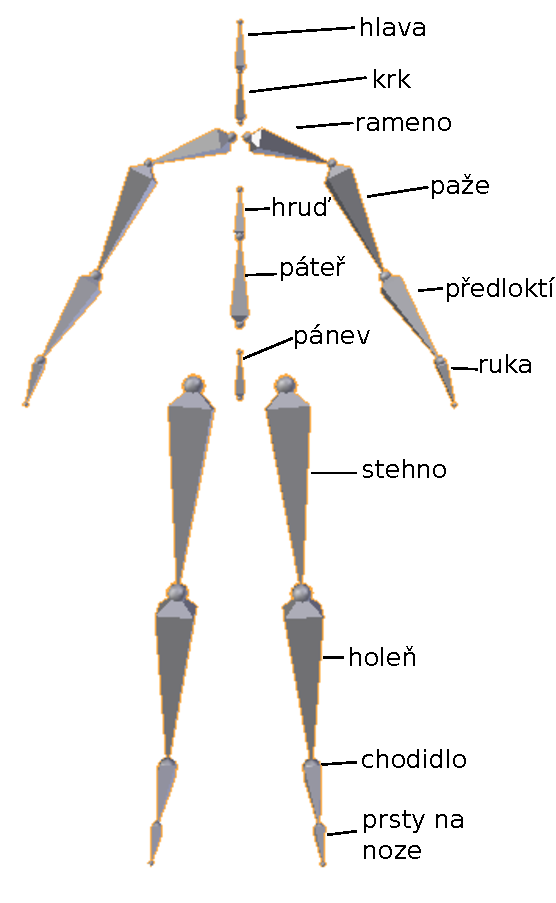
\includegraphics{fig/skeleton_names.pdf}}
\caption{Kostra, která je vytvořena a použita v této práci.} \label{bone_structure}
\end{center}
\end{figure}

Každá kost má lokální transformaci: posunutí, rotaci a zvětšení. Tato transformace se může uložit jako matice a určuje transformaci vůči rodičovské kosti, pokud existuje. Pro realistické modely člověka se většinou používá pouze rotace. Výsledná globální transformace kosti se získá kombinací rodičovské globální transformace a vlastní lokální transformace. Globální transformace všech kostí se vypočítá procházením stromové struktury kostry a~postupným násobením transformačních matic od kořene k listům. Pro kořenovou kost je lokální transformace její globální. 

Před připojením kůže na kostru se kostra nastaví do pozice nazývané \textit{bind pose} \cite{bindPose}. To je základní pozice kostry před jakýmkoliv pohybem. V tuto chvíli se na kostru připojí kůže. Následně jsou určeny a uloženy bind pose matice $\mathbf{B}$ pro každou kost. Ty určují jejich transformaci z počátku souřadného systému kostry do bind pose. Matice $\mathbf{B}_a$ každé kosti určuje její aktuální transformaci z počátku souřadného systému kostry. Před prvním pohybem kostry jsou shodné s $\mathbf{B}$. Chceme-li změnit pózu kostry (matici $\mathbf{B}_a$ nějaké kosti) a tím i připojené kůže, musí se vrcholy transformovat ze souřadného systému kůže do~souřadného systému kostry. K tomu se použije \textit{inverzní bind pose matice} $\mathbf{B}_i$. Ta určuje transformaci kosti potřebnou pro přesun kosti z bind pose do počátku souřadného systému. Tedy invertuje transformaci, která byla na kůži aplikována v bind pose. Matematický zápis transformace $\mathbf{T}$ (obrázek \ref{transform_pose}) určující novou pozici kosti je následující:
\begin{eqnarray}
\mathbf{T} &=& \mathbf{B}_i \mathbf{B}_a\label{r.transform_mat}
\end{eqnarray}
Poté se může použít $\mathbf{T}$ na výpočet nové pozice vrcholů kůže. Vrchol bude pořád ve stejné relativní pozici vůči kosti. Transformování se často provádí na grafické kartě ve vertex shaderu.
 \begin{figure}[h]
\begin{center}
\scalebox{0.5}{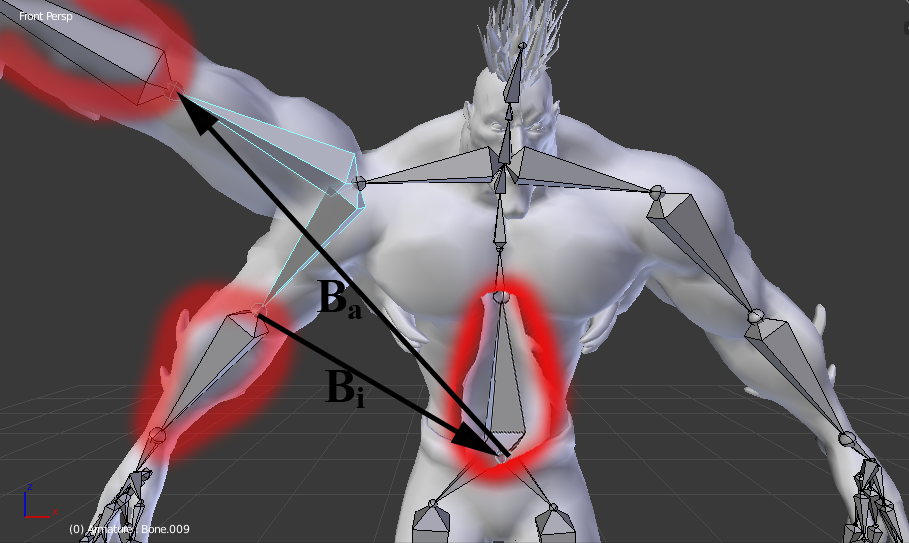
\includegraphics{fig/transform_pose.png}}
\caption{Transformace předloktí. Prvně se aplikuje inverzní bind pose matice a poté aktuální transformace kosti. Model byl převzat z \cite{venom}.} \label{transform_pose}
\end{center}
\end{figure}
\section{Skinning}
Skinning \cite{skinningMethods} je nazýván proces přidělování kostí vrcholům kůže a určování jejich vah. Tento proces může probíhat algoritmicky nebo ručně v některém z modelovacích programů. Nejjednodušší způsob přiřazení kůže ke kostře je každé kosti přiřadit samostatný pevný objekt, jako je např. válec. Na každý takový objekt se poté aplikuje transformace přiřazené kosti. Tento přístup není vhodný pro realistické animování.

Pokročilejší, ale stále základní metoda je \textit{Jednoduchý skinning}, který již používá kůži, tedy jeden model pro celou kostru. Přiřazuje jeden vrchol k jedné kosti. Každý vrchol se poté transformuje podle přiřazené kosti. Je používán například ve starších hrách. Je dobře použitelný pro modely s nízkým počtem trojúhelníků. U detailnějších modelů způsobuje nepěkné deformace v kloubech a animace vypadá nepřirozeně. 

\subsection{Linear blend skinning} \label{linear_blend_skinning}
\textit{Linear blend skinning} \cite{skinningMethods} je modernější algoritmus. Je nepublikovaný a vyskytuje se i~pod jinými názvy, jako je \textit{skeleton-subspace deformation}, \textit{enveloping} nebo pouze \textit{skinning}. Každému vrcholu umožňuje přiřazení více kostí. Každá dvojice kost a vrchol má přiřazenou váhu. Váha určuje jak velký vliv má pohyb konkrétní kosti na výslednou pozici vrcholu. Na~vstupu očekává následující data: 
\begin{itemize}
\item Kůže v bind pose, typicky reprezentovaná jako polygonální model. Propojení mezi vrcholy se v průběhu nemění, pouze pozice vrcholů. 
\item Transformace kostí, reprezentované jako matice $\mathbf{T}_1,\ldots,\mathbf{T}_m$ určené podle rovnice \ref{r.transform_mat}. Tyto matice jsou typicky jediná veličina, která se v průběhu animace může měnit. 
\item \label{weight_sum} Váhy vrcholů, pro každý vrchol $\mathbf{v}_i$ máme váhy $w_{i,1},\ldots,w_{i,m} \in \mathbb{R}$. Každá váha $W_{i,j}$ určuje vliv kosti $j$ na vrchol $i$. Celkový součet všech vah je 1, přičemž žádná váha není záporná. 
\end{itemize}
Množství kostí ovlivňující jeden vrchol se může významně lišit (např. od 1 do 10). Kvůli limitacím grafického hardwaru se často uvažuje že jich není více než 4. Transformovaná pozice vrcholu $\mathbf{v}'_i$ se určí podle následující rovnice:
\begin{eqnarray}
\mathbf{v}'_i &=& \Bigg(\sum_{j=1}^mw_{i,j} \mathbf{T}_j\Bigg)\mathbf{v}_i\label{r.linear_blend_skinning}
\end{eqnarray}
 Tato metoda podává dobré výsledky, pokud míchané transformace nejsou příliš rozdílné. Problémy nastávají jestliže potřebujeme míchat transformace, které se významně liší v jejich rotaci. Z lineární kombinace rotací nevzniká rotace. To je důsledkem faktu, že Lieova grupa 3D transformací, $SO(3)$, není lineární prostor, ale zakřivená varieta. Pokud jsou si rotace blízké není to problém. Uvažujme ale tyto dvě rotace.
$$\mathbf{R}_1\left[\begin{array}{ccc}
1 & 0 & 0\\
0 & 1 & 0\\
0 & 0 & 1~\end{array}\right], \quad \mathbf{R}_2 \left[\begin{array}{ccc}
-1 & 0 & 0\\
0 & -1 & 0\\
0 & 0 & 1~\end{array}\right]$$ 

Matice $\mathbf{R}_1$ je maticí identity a matice $\mathbf{R}_2$ je rotace okolo osy Z o 180 stupňů. Lineární míchání $0.5 \cdot \mathbf{R}_1 + 0.5 \cdot \mathbf{R}_2$ nám dá za výsledek matici hodnosti 1, která promítá 3D prostor na osu Z. To má za následek ztrátu objemu modelu. Velké relativní rotace nejsou vzácné, protože klouby jako ramena a zápěstí mají velký rozsah pohybu. Tyto problémy je možné řešit zavedením více parametrů než má linear blend skinning. Takové metody se nazývají \textit{multilineární}. Tyto metody ale nemusí být žádoucí kvůli nutnosti vytvářet a ukládat více vah pro každý vrchol.

\subsection{Dual quaternion skinning}
Velmi rozšířenou metodou je nelineární metoda \textit{Dual quaternion skinning} \cite{dualQuat}, kde se místo matic míchají \textit{duální kvaterniony}. Tato metoda zachovává objem modelu, řeší artefakty vznikající u linear blend skinning a je velmi rychlá. Používá se v rozšířených modelovacích programech jako je např. Blender. Klasické kvaterniony umožňují reprezentovat 3D rotaci okolo osy. Tato osa ale musí procházet počátkem souřadného systému. Oproti tomu duální kvaterniony toto omezení nemají - osa může být libovolná. Kromě toho duální kvaterniony umožňují popsat posunutí. Ale neumožňují popsat změnu měřítka. Proto nemůže docházet ke ztrátě objemu jako u matic, kde násobením může vznikat zmenšení. Duální kvater\-niony jsou také výhodné pro GPU hardware, protože obsahují méně hodnot než matice. Pro porovnání metod viz obrázek \ref{skinning_methods}.

\begin{figure}[h]
\begin{center}
\scalebox{0.5}{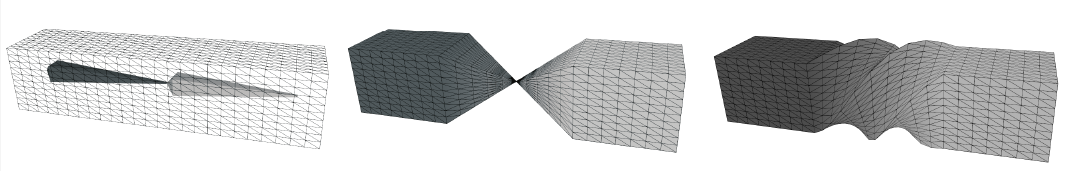
\includegraphics{fig/dual_quat.png}}
\caption{Zleva doprava: model v bind pose, linear blend skinning a dual quaternion skinning. Převzato z \cite{skinningMethods}.} \label{skinning_methods}
\end{center}
\end{figure}

\subsection{Metoda obálek}
Přiřazení vah je možné automaticky \textit{metodou obálek} \cite{envelopes}. Tato metoda je založena na blízkosti kostí a jejich geometrie. Každá kost má dvě oblasti vlivu. Vnitřní oblast, kde je geometrie plně ovlivněna touto kostí. A vnější oblast, kde je geometrie méně ovlivněna kostí, čím blíže je k okraji této oblasti. 
Pokud chceme mít váhy určené kvalitně, je nutné nastavit váhy ručně. To je možné v některém modelovacím programu, například Blender poskytuje \textit{Weight Paint} mód, kde se pohybem štětce po modelu určují váhy vrcholů pro jednotlivé kosti. Tento proces je iterativní a náročný. Kreslením se odebírají nebo přidávají váhy vrcholům pro jednu aktivní kost. Poté se zkouší efekt na známé póze, upravují a vyhlazují váhy a tento proces se opakuje, dokud výsledek není dostatečně přirozený. Na obrázku \ref{envelope_weight_paint} je ukázána obálka a model ve Weight Paint módu.
\begin{figure}[h]
\begin{center}
\subfloat{{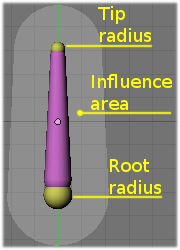
\includegraphics[width=3cm]{fig/envelopes.png}}}
\qquad
\subfloat{{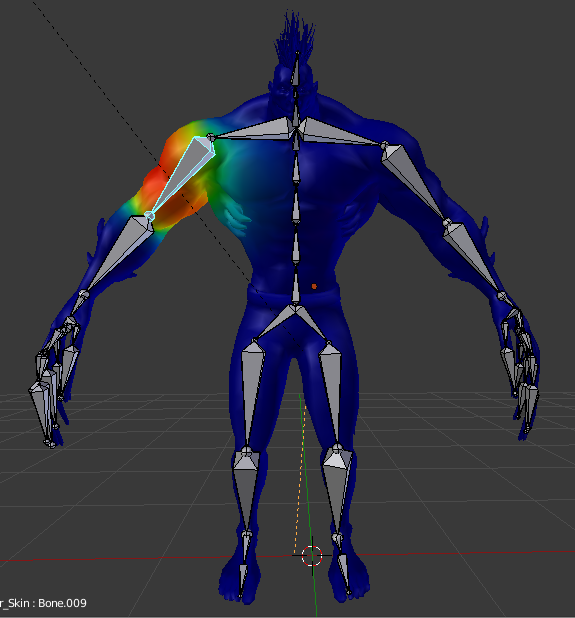
\includegraphics[width=7cm]{fig/weight_paint.png}}}
\caption{Metoda obálek v programu Blender (převzato z \cite{envelopes}) a model \cite{venom} ve Weight paint módu v Blenderu.} \label{envelope_weight_paint}
\end{center}
\end{figure}

\section{Tvorba animace}
Animace člověka se vyskytuje ve velkém množství aplikací v různých prostředích a podmínkách. Tyto animace by proto měly být přizpůsobitelné prostředí v reálném čase. Také by měly působit přirozeně a tím přidávat na reálnosti. Základní nástroje pro specifikaci pohybu jsou založeny na \textit{kinematikách}. Existují dva způsoby popisu kinematické informace: \textit{inverzní} a \textit{přímá kinematika}, viz kapitola \ref{kinematics}. 

Welbergen a spol. \cite{survey} dělí techniky tvorby animace do tří skupin: \textit{procedurální animace}, \textit{fyzikálně založená simulace} a \textit{editace pohybu}. Techniky se také mohou kombinovat dohromady a využívat vhodnější techniku pro danou situaci nebo část těla. Může se například použít technika editace pohybu dokud nedojde k interakci s prostředím a ta se může zpracovat pomocí fyzikálně založené simulace. Nebo pomocí procedurální animace vytvořit gesta rukou a fyzikální simulací zachovat fyzikálně přirozené balancování spodní části těla.

\subsection{Procedurální animace}
Procedurální animace popisuje animaci algoritmicky pomocí matematických vzorců. Její úspěch závisí na tom, jak hluboce jsme schopni pochopit a modelovat simulovaný pohyb. Metody mohou popisovat rotace kostí přímo nebo popisovat cesty koncových uzlů kostry (chodidla), potom se používá inverzní kinematika. 

Procedurální animace umožňuje přesné časování a pozicování končetin a může využívat velké množství parametrů, pomocí kterých je možné upravit výstup na míru požadavkům. Dobře se adaptují na prostředí a jsou málo výpočetně náročné. Nicméně je často problematické zakomponovat detaily jako jsou u editace pohybu do matematického popisu. Také je nutné explicitně zachovávat fyzikální přirozenost v procedurálním modelu pohybu pro všechny možnosti parametrů. Je často používána pro animaci gest a mluvení, které vyžadují velké množství parametrů.

\subsection{Fyzikálně založená simulace}
V mnoha případech je vhodné počítat s \textit{dynamikami} \cite{surveyWalk}, aby byla zachována realističnost pohybu. Tyto případy mohou být:
\begin{itemize}
\item jestliže postava nese náklad
\item jestliže postava musí reagovat na externí síly jako poryvy větru
\item  povrch na kterém se pohybuje je komplexní (schody atp.)
\end{itemize}

Dynamiky se používají u technik ze skupiny fyzikálně založené simulace. Dynamiky jsou založené na Newtonových pohybových zákonech. Spojují síly (resp. točivé momenty rotací) do výsledného pohybu (resp. rotace) podle rovnice: 
\begin{eqnarray}
f=m \cdot \ddot{x}\label{r.dynamics1}
\end{eqnarray}
kde $f$ je síla aplikovaná na objekt, $m$ je jeho hmotnost, $\ddot{x}$ je druhá derivace $x$ podle času. Pro rotace vypadají rovnice podobně. Točivé momenty a úhlové pozice jsou spojeny pomocí:
\begin{eqnarray}
t=i \cdot \ddot{\theta} + \dot{\theta} \times i \cdot \ddot{\theta}\label{r.dynamics2}
\end{eqnarray} 
kde $t$ je točivý moment, $i$ je matice setrvačnosti, $\dot{\theta}$ je úhlová rychlost a $\ddot{\theta}$ je úhlové zrychlení. \textit{Přímá dynamika} je aplikace těchto zákonů k výpočtu pohybu vygenerovaného danou silou. \textit{Inverzní dynamika} se zabývá určováním síly, která by vygenerovala daný pohyb.

Ve fyzikálně založené simulaci je model typicky reprezentovaný jako systém pevných těles propojených klouby. Každé z těchto pevných těles má přiřazené fyzikální vlastnosti jako např. hmotnost. Pohyb je generován manipulací s točivými momenty kloubů s použitím přímé dynamiky. Pro umožnění kolizí je nutné geometricky reprezentovat pevná tělesa. Použití samotného povrchového modelu je příliš výpočetně náročné, proto se pro kolize používají aproximace pomocí základních tvarů (např. válec).

Metody mohou fungovat na základě zadávání geometrických omezení jako parametrů animace. Tato omezení mohou být typicky splněna velkým množstvím různých točivých momentů. Proto se mohou zavést objektivní funkce pro preferenci jistých řešení. Tyto metody jsou pro animace v reálném čase velmi pomalé. Jiný způsob je používání kontrolérů, do kterých vstupuje žádaný stav systému. Výstupem je množina točivých momentů kloubů, které po aplikaci na systém vedou proměnné k jejich požadovaným hodnotám. Kontrolér využívá fyzikálních vlastností pohybujícího se těla. Úlohou kontroléru je minimalizace nesrovnalostí mezi aktuálním a požadovaným stavem. Síly a točivé momenty určené kontrolérem, gravitace a síly způsobené externími vlivy, jsou aplikované na fyzické tělo. To je poté pohnuto pomocí přímé dynamiky. 

Fyzikálně založená simulace poskytuje fyzikálně realistický pohyb a interakci s prostředím. Umožňuje zachování parametrů pod vlivem externích sil. Nicméně přesné časování a umisťování končetin je problematické. Ačkoliv fyzikální simulace poskytuje fyzikálně správný pohyb, není často dostačující pro vytvoření přirozeného pohybu. 

\subsection{Editace pohybu}
Metody editace pohybu vytváří pohyb na základně vzorů pohybu. Metody modifikace pohybu generují nová pohybová primitiva modifikací jednoho vzoru pohybu. Kombinační techniky vytváří pohybová primitiva pomocí databáze většího množství vzorových primitiv. Pohyby se mohou vytvářet pomocí technik ze zpracování signálů, interpolací mezi vzory pohybů nebo pomocí statistických modelů. 

Techniky editace pohybu zachovávají přirozenost vstupních vzorů pohybu, ale pouze jsou-li změny malé. Přirozenost i při větších změnách je zachována technikami používajícími více vzorů na jeden pohyb. Nicméně, pro všechny techniky roste počet vzorů  exponenciálně s~počtem parametrů animace. Navíc techniky editace pohybu neposkytují fyzikální interakci s prostředím, ale jsou vázány na specifický kontext. Jsou vhodné pro vytváření animací v~předstihu pro neinteraktivní aplikace (např. filmy). Pro interaktivní (např. videohry) je potřeba velká databáze pohybů. Pohyby se mohou vytvářet pomocí technik ze zpracování signálů, interpolací mezi vzory pohybů nebo pomocí statistických modelů.

Vstupní data mohou být být tvořená animátorem ručně, ale mohou být získána i např. pomocí \textit{motion capture}. Motion capture  \cite{motion_capture} jsou techniky pro nahrávání pohybů člověka, zvířete nebo jiného subjektu. Mají velké využití ve filmech a videohrách. Nejčastěji se používá optických metod pro zachycení pohybu. V Motion capture má herec okolo každého kloubu značky, které jsou zaznamenávány a sledovány kamerami, viz obrázek \ref{motion_capture_img}. Výstupem je množina lokací bodů v čase. Těmi se poté proloží kostra.
\begin{figure}[h]
\begin{center}
\scalebox{0.4}{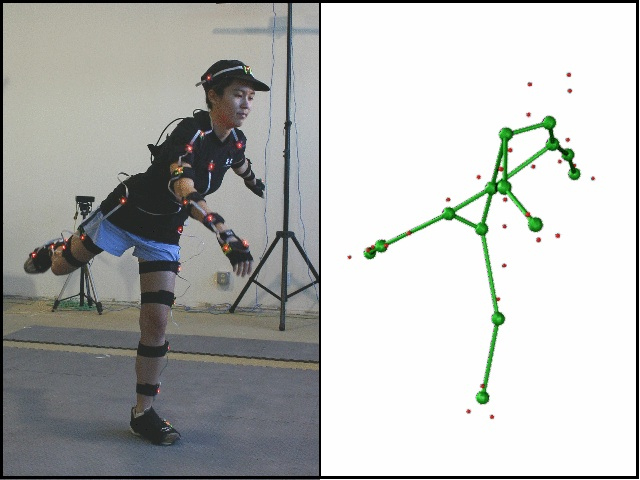
\includegraphics{fig/motion_capture.jpg}}
\caption{Automatická rekonstukce kostry podle pozic značek. Převzato z \cite{motion_capture}.} \label{motion_capture_img}
\end{center}
\end{figure}

\chapter{Kinematiky} 
\label{kinematics}
Kinematiky v počítačové grafice slouží pro manipulaci s kostrou. Jsou  rozděleny na dvě části -- přímá a inverzní kinematika. V přímé kinematice se hýbe s každou kostí v řetězci kostí a podle toho se určí výsledná pozice posledního článku -- \textit{koncového efektoru}. Výsledky při ručním vytváření animace jsou velmi závislé na schopnostech animátora, protože musí nastavovat pozice kostí od ruky. V této technice je obtížné omezovat pohyb, například že~chodidlo nemůže proniknout do země. 

Máme-li \textit{řetězec kloubů}, kde každý kloub $i$ má přiřazen úhel $\theta_i$, který určuje jeho rotaci oproti jeho předkovi, viz obrázek \ref{ik_chain}. Potom stav řetězce je určen stavovým vektorem $\boldsymbol{\theta}(\theta_1,\dots,\theta_n)$. Označme pozici koncového efektoru $\mathbf{P}$. Přímá kinematika řeší následující rovnici:
\begin{eqnarray}
\mathbf{P} = f(\boldsymbol{\theta})\label{r.forward_kinematics}
\end{eqnarray}
Každý kloub může mít více než jeden \textit{stupeň volnosti}, tedy být definován více úhly. Tím je určena složitost struktury kloubů, která je definována jako součet stupňů volnosti všech prvků.

Oproti tomu v inverzní kinematice \cite{Buss09introductionto,welman} se hýbe pouze s koncovým efektorem a pohyb ostatních kloubů se dopočítá, tak aby byl tento pohyb umožněn. To je matematicky zapsáno následovně:
\begin{eqnarray}
\boldsymbol{\theta} = f^{-1}(\mathbf{P})\label{r.inverse_kinematics}
\end{eqnarray}

\begin{figure}[h]
\begin{center}
\scalebox{0.4}{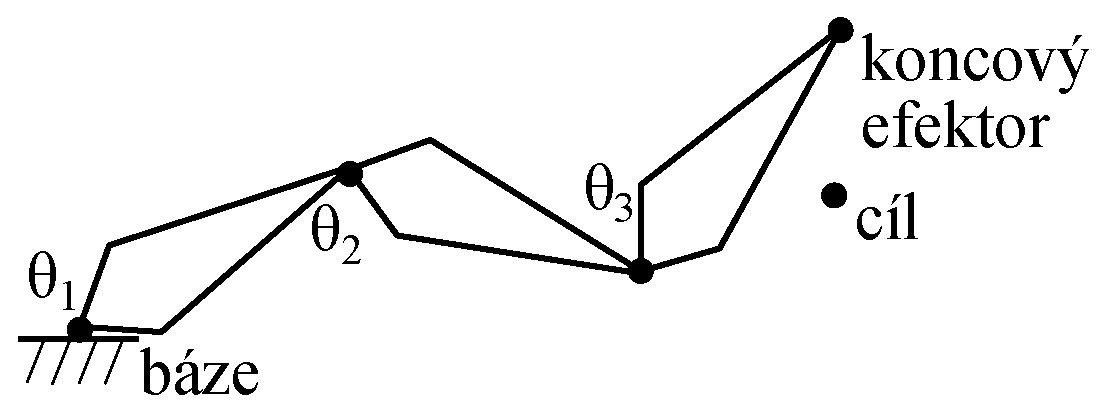
\includegraphics{fig/ik_chain.eps}}
\caption{Příklad řetězce tří kloubů.} \label{ik_chain}
\end{center}
\end{figure}
Řešení inverzní kinematiky není tak jednoduché jako přímé. Funkce $f$ je nelineární a~ačkoliv v~rovnici \ref{r.forward_kinematics} existuje unikátní namapování z $\boldsymbol{\theta}$ na $\mathbf{P}$, pro inverzní mapování v~rovnici \ref{r.inverse_kinematics} může být nekonečné množství $\boldsymbol{\theta}$ pro jedno konkrétní $\mathbf{P}$. Analytické řešení pro libovolný řetězec kloubů neexistuje. Problém se řeší pomocí numerických metod pro řešení systémů nelineárních rovnic. Z nekonečného množství řešení je snaha vybírat to nejvhodnější řešení. Různé metody preferují různé řešení a proto se metody vybírají na základě konkrétně řešeného problému. V případě lidské kostry má každý kloub určené stupně volnosti, aby rotovali jenom v určitých směrech a také je definován maximální úhel rotace. Například koleno rotuje pouze v jednom směru a nemůže být otevřeno více než 180 stupňů a zavřeno méně než 30 stupňů. Inverzní kinematika poskytuje lepší kontrolu nad koncovým efektorem, jehož cílová pozice nás většinou nejvíce zajímá. V modelovacím programu můžeme hýbat např. pouze chodidlem a nemusíme také pohybovat stehenní a lýtkovou kostí. Toho se také využije v procedurální animaci lidské chůze, kde budeme určovat trajektorie koncových efektorů. Techniky založené na kinematikách využívají empirickou a biomechanickou znalost pohybu pro generování animace. 

Nyní si ukážeme některé způsoby řešení inverzní kinematiky.
\section{Jacobiho inverzní metoda}
\textit{Jacobiho inverzní metoda} \cite{Buss09introductionto, welman, AristidouTR632} je iterativní metoda využívající \textit{Jacobiho matice} k~aproximaci řešení. Vztah mezi kartézským prostorem koncového efektoru $\mathbf{P}$ a prostoru kloubů úhlů $\boldsymbol{\theta}$ je:
\begin{eqnarray}
\mathbf{\dot{P}} = J(\boldsymbol{\theta})\boldsymbol{\dot{\theta}}\label{r.jacobian_vztah}
\end{eqnarray}
kde tečka značí první derivaci podle času. Jacobiho matice $J$ je $m \times n$ matice:
\begin{eqnarray}
J(\boldsymbol{\theta}) = \bigg(\frac{\partial P_i}{\partial \theta_j}\bigg)_{i,j}\label{r.jacobian_matrix}
\end{eqnarray}
kde $m$ je počet dimenzí pozice koncového efektoru $\mathbf{P}$, $n$ je počet dimenzí $\boldsymbol{\theta}$, $i = 1,\dots,m$ a~$j = 1,\dots,n$. $J$ je matice částečných derivací celého řetězce relativně ke koncovému efektoru. $J$ mapuje změny proměnných kloubů $\boldsymbol{\theta}$ na změny v pozici koncového efektoru. Sloupec $i$ v~$J$ reprezentuje inkrementální změnu pozice koncového efektoru způsobenou inkrementální změnou proměnné $\theta_i$. 
Neznámou pro inverzní kinematiku je $\boldsymbol{\dot{\theta}}$, proto potřebujeme inverzi Jacobiho matice. Vztah je následující:
\begin{eqnarray}
\boldsymbol{\dot{\theta}} = J^{-1}(\boldsymbol{\theta})\mathbf{\dot{P}}\label{r.jacobian_vztah_inverse}
\end{eqnarray}
Poté co určíme Jacobiho matici, hledáme hodnotu $\Delta\boldsymbol{\theta}$ pro inkrementaci $\boldsymbol{\theta}$:
\begin{eqnarray}
\boldsymbol{\theta} = \boldsymbol{\theta} + \Delta\boldsymbol{\theta}\label{r.jacobian_increment}
\end{eqnarray}
Změna v pozici koncového efektoru určená touto změnou je:
\begin{eqnarray}
\Delta\vec{\mathbf{s}} \thickapprox J\Delta\boldsymbol{\theta}\label{r.jacobian_change}
\end{eqnarray}
Hodnota $\Delta\boldsymbol{\theta}$ by měla být vybrána tak, aby $\Delta\vec{\mathbf{s}}$ přibližně odpovídala $\vec{\mathbf{e}}$ -- rozdílu mezí cílovou a aktuální pozicí koncového efektoru. Potom přímá kinematika může být přepsána jako $\vec{\mathbf{e}} = J\Delta\boldsymbol{\theta}$ a inverzní jako $\Delta\boldsymbol{\theta} = J^{-1}\vec{\mathbf{e}}$.

Jacobiho matice ale není vždy invertibilní, tzn. není čtvercová a zároveň singulární. To nastane když konfigurace kloubů je redundantní nebo když prochází skrz nebo blízko singulární konfigurace.

Řetězec kloubů je redundantní jestliže obsahuje více stupňů volnosti, než je potřeba pro specifikaci cíle koncového efektoru. Je-li cíl koncového efektoru určen pozicí v 3D prostoru, potom jakýkoliv řetězec obsahující více než 3 stupně volnosti je redundantní a tedy existuje nekonečně mnoho řešení. Jacobiho matice potom má více sloupců než řádků. V takových případech se $J^{-1}$ nahradí generalizovanou inverzí $J^{\dagger}$, vetšinou \textit{Moore-Penroseovou pseudoinverzí}. Jestliže existuje nekonečné množství řešení, je možné toho využít pro splnění nějakého sekundárního kriteria, např. vyhnutí se překážkám.
Matice je singulární jestliže dva nebo více řádků jsou lineárně závislé, příklad takové konfigurace je vidět na obrázku \ref{singular}. Jacobiho matice pro takovou konfiguraci bude obsahovat nuly v prvním řádku a nemůže být invertována. V takovém případě je možné použít pseudoinverzní matici, která poskytne řešení v singulární konfiguraci, nicméně v okolí singulární konfigurace bude nevhodně oscilovat. 
\begin{figure}[h]
\begin{center}
\scalebox{0.4}{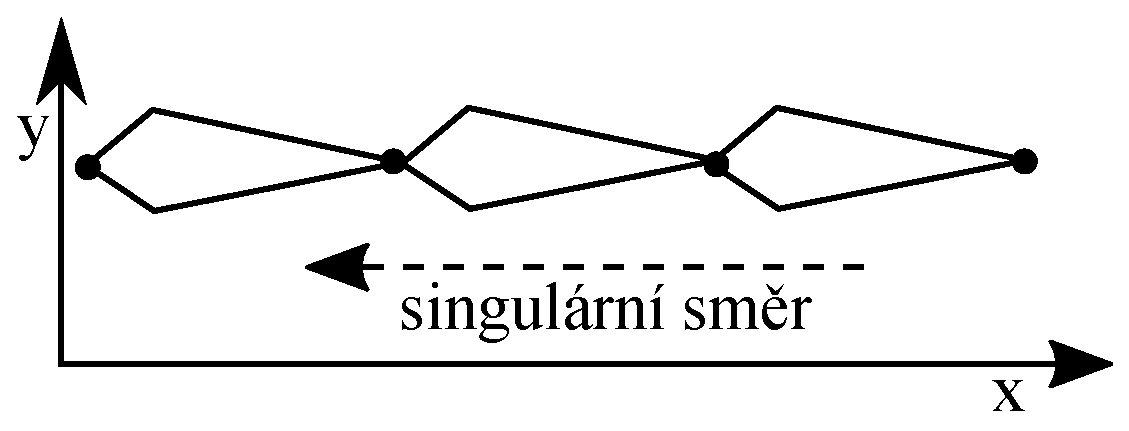
\includegraphics{fig/singular.eps}}
\caption{Singulární konfigurace řetězce kloubů.} \label{singular}
\end{center}
\end{figure}
\section{Cyclic Coordinate Descent} \label{ccd}
\textit{Cyclic Coordinate Descent} (CCD) \cite{welman} je řešení inverzní kinematiky založené na iterativním heuristickém vyhledávání, které se snaží o minimalizaci rotační chyby  zpracováváním jednoho kloubu v jeden okamžik. Každá iterace provede jednotlivě pohyb všech článků od~nejposlednějšího k prvnímu. To se opakuje dokud se nedosáhne požadované pozice koncového efektoru a nebo dokud se nepřesáhne maximální počet cyklů. K určení úhlu rotace se používají dva vektory. Protože metoda pracuje s jedním kloubem v jeden okamžik, zvýhodňuje klouby na začátku. Oproti metodám používající Jacobiho matice provádí více iterací. Ačkoliv je algoritmus jednoduchý, je často nutné ho dále přizpůsobovat, aby bylo dosaženo vhodných výsledků.

Mějme iteraci $i$ (viz obrázek \ref{ccd_img}) a pozici kloubu $\mathbf{k}_i$ pro $i$-tý kloub od konce řetězce. Potom vektor $\mathbf{P}_{ia}$ je vektor od pozice kloubu $\mathbf{k}_i$ k aktuální pozici koncového efektoru a $\mathbf{P}_{ip}$ je vektor od $\mathbf{k}_i$ do požadované pozice koncového efektoru. Budeme-li rotovat vektor $\mathbf{P}_{ia}$ o úhel $\phi$, dostaneme nový vektor $\mathbf{P}'_{ia}(\phi)$. Jestliže úhel bude nabývat libovolných hodnot, $\mathbf{P}'_{ia}(\phi)$ začne tvořit kruh se středem $\mathbf{k}_i$. Bod na tomto kruhu nejblíže k požadované pozici $\mathbf{P}_p$, je bod, na kterém kruh protíná přímku určenou vektorem $\mathbf{P}_{ip}$. Proto budeme měnit rotaci kloubu $\mathbf{k}_i$ tak, aby se $\mathbf{P}_{ip}$ a $\mathbf{P}'_{ia}(\phi)$ zarovnaly.
\begin{figure}[h]
\begin{center}
\scalebox{0.4}{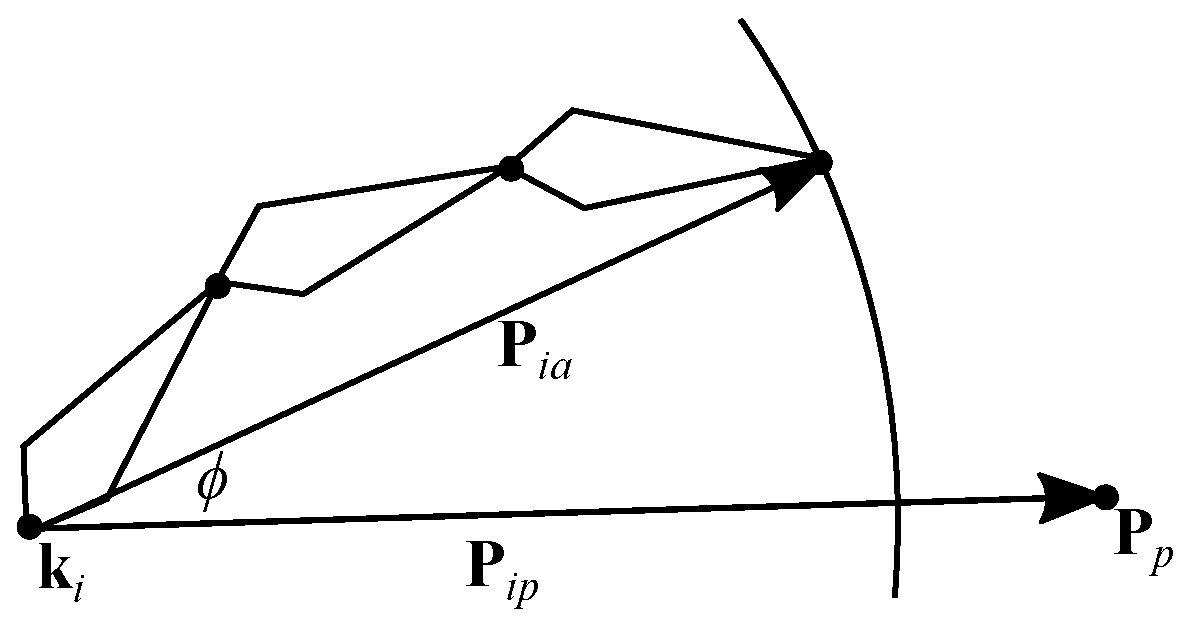
\includegraphics{fig/ccd.eps}}
\caption{Ukázka jedné iterace metody CCD.} \label{ccd_img}
\end{center}
\end{figure}
Úhel $\phi$ který hledáme, je úhel, který maximalizuje následující funkci:
\begin{eqnarray}
g(\phi) &=& k_1(1 - \cos\phi) + k_2 \cos\phi + k_3 \sin\phi\label{r.ccd_max1}
\end{eqnarray}
kde $k_1$, $k_2$ a $k_3$ jsou konstantní koeficienty, pro detaily viz \cite{welman}. Funkce má maximum v~intervalu $-\pi \leq \phi \leq \pi$, když je první derivace nula a druhá derivace je záporná. Z první podmínky dostáváme rovnici:
\begin{eqnarray}
\phi &=& \tan^{-1}\frac{k_3}{k_2 - k_1}\label{r.ccd_max2}
\end{eqnarray}
která vymezí kandidátní hodnotu $\phi_c$ v rozsahu $\frac{-\pi}{2} \leq \phi_c \leq \frac{\pi}{2}$. Protože $\tan$ je periodické, musíme uvažovat i dvě další kandidátní hodnoty: $\phi_c + \pi$ a $\phi_c - \pi$. Z kandidátních hodnot se vybere taková, která spadá do intervalu $-\pi \leq x \leq \pi$ a jejíž druhá derivace je záporná. Je-li jich více, funkce se vyhodnotí nad všemi a vybere se z nich maximum. Poté co jsme získali úhel $\phi$, můžeme ho vynásobit váhou určující tuhost kloubu a přičíst ho k aktuální rotaci $r_i$ kloubu $i$. Poté se pokračuje s iterací $i+1$.

\chapter{Lidská chůze}
Lidská chůze \cite{gait_review} se skládá z opakujících se \textit{krokových cyklů} neboli \textit{dvojkroků}, viz obrázek \ref{gait_cycle}. Cyklus je sekvence pohybů od doby, kdy se jedna noha dotkne země, do doby kdy se stejná noha dotkne země znovu. Každý krokový cyklus má dvě základní fáze: \textit{stojnou fázi} a \textit{švihovou fázi}. Protože je cyklus shodný pro obě nohy, budeme popisovat pouze jednu.

Stojná fáze, je fáze, kdy je noha v kontaktu se zemí. Zabírá 60\% dvojkroku a začíná s~\textit{úderem paty} (\textit{počáteční kontakt}) a končí s \textit{odrazem palce}. Je dále rozdělena do podfází:
\begin{itemize}
\item \textit{stádium zatěžování}
\item \textit{mezistoj}
\item \textit{konečný stoj}
\item \textit{předšvihová fáze}
\end{itemize}
Po počátečním kontaktu pravé nohy nastává perioda \textit{dvojí opory}, která končí při odrazu palce levé nohy. Následuje \textit{jedno-oporová fáze} do té doby, než se levá dostane do počátečního kontaktu. Nastává druhá perioda dvojí opory, až do odrazu palce pravé nohy. V~každé fázi dvojí opory je jedna noha vpředu, právě se dotkla země. A druhá je vzadu připravena na zvednutí se ze země. Přední noha je ve stadiu zatěžování  a zadní je v konečném švihu. V~každém krokovém cyklu jsou dvě periody dvojí opory a dvě periody jedno-oporové fáze. Dvojí opora zabírá přibližně 10\% dvojkroku, ale její délka se mění s rychlostí chůze. S větší rychlostí se prodlužuje švihová fáze a zkracuje fáze dvojí opory. Když dvojí opora úplně vymizí, z chůze se stává běh. Mezi kroky běhu je fáze letu, kdy není žádná noha na zemi.

Švihová fáze nastává, když je chodidlo ve vzduchu a trvá 40\% délky dvojkroku. Začíná s úderem paty a končí s druhým odrazem palce.  Je dále rozdělena do podfází:
\begin{itemize}
\item \textit{počáteční švih}
\item \textit{mezišvih}
\item \textit{konečný švih}
\end{itemize}

\begin{figure}[h]
\begin{center}
\scalebox{0.4}{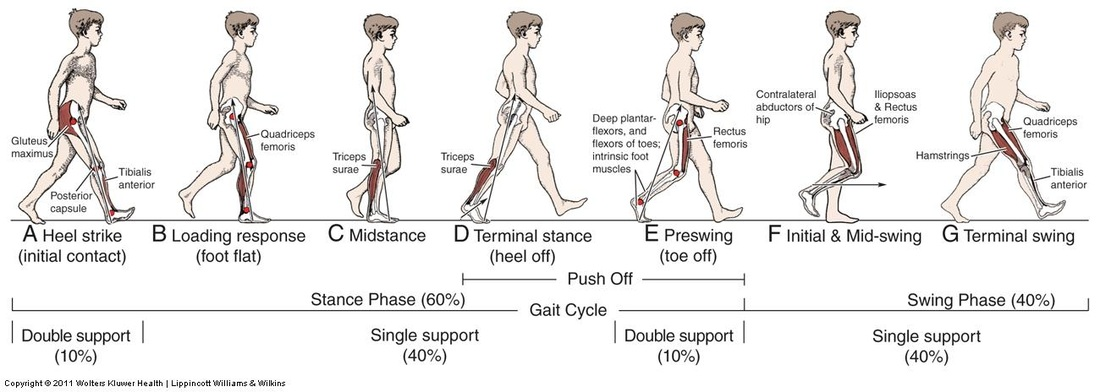
\includegraphics{fig/gait-cycle.jpg}}
\caption{Krokový cyklus a jeho fáze. Převzato z \cite{gait_img}.} \label{gait_cycle}
\end{center}
\end{figure}

Nyní si popíšeme některé termíny a parametry specifikující chůzi (obrázek \ref{step_length}). \textit{Délka dvojkroku} je vzdálenost mezi dvěma po sobě jdoucími kroky stejné nohy. Skládá se ze dvou délek kroku -- levé a pravé. Každá s nich určuje vzdálenost o kterou se jedna noha přesune před druhou. Může být např. nulová, když se levá noha přesune na úroveň pravé a ne před ní. \textit{Šířka dvojkroku} je vzdálenost mezi přímkami určenými středy pat obou nohou při chůzi. \textit{Úhel vytočení chodidla} určuje úhel mezi zmíněnou přímkou a přímkou procházející středem chodidla. \textit{Kadence} je počet kroků v daném čase. V jednom krokovém cyklu jsou dva kroky a~tedy kadence je měřítko půl-cyklů. Čas dvojkroku $c$ v sekundách se určí jako $c = 120/kad$, kde $kad$ je kadence v krocích za minutu. \textit{Rychlost chůze} je vzdálenost ušlá v čase. Okamžitá rychlost je variabilní v průběhu kroku, ale průměrná rychlost je výsledkem kadence a délky dvojkroku. Rychlost chůze $r$ se spočítá jako $r = d/c$, kde $d$ je délka dvojkroku. Rychlost chůze tedy závisí na délce kroku, které závisí na délce švihové fáze.

\begin{figure}[h]
\begin{center}
\scalebox{0.4}{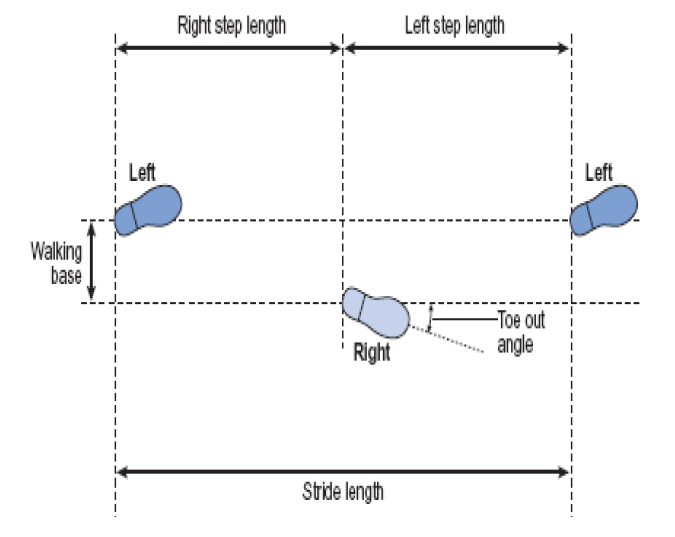
\includegraphics{fig/step_length.png}}
\caption{Délka kroku, šířka kroku a úhel vytočení chodidla. Převzato z \cite{gait_review}.} \label{step_length}
\end{center}
\end{figure}

\section{Fáze krokového cyklu}
Tato sekce obsahuje podrobný popis jednotlivých fází krokového cyklu. Každá z osmi fází má funkční objektiv. Sekvenční kombinace fází umožňuje končetině dosáhnout tří základních úkolů. Úkoly jsou přesun hmotnosti těla, jednooporová fáze a posun končetiny ve švihové fázi. Pro tuto podkapitolu bylo čerpáno z \cite{gait_review}. 
\subsection{Počáteční kontakt}
V této fázi je kyčel ohnutá, koleno natažené a kotník v neutrální poloze. Kontakt se zemí je dosažen pomocí paty, která se stává středem otáčení. Druhá noha je na konci konečného stoje. Tato fáze obsahuje moment kdy právě nastane dotyk nohy se zemí. Držení těla v tuto chvíli určuje pohyb končetiny ve stádiu zatěžování. 
\subsection{Stádium zatěžování}
Stádium zatěžování je fáze, kde je váha těla přenesena na přední nohu. Koleno je pokrčeno pro absorbování šoku. Chodidlo se dostává do plného kontaktu se zemí. Protilehlá noha je v~předšvihové fázi. Tato fáze je počátkem fáze dvojí opory. Pokračuje dokud nezačne být druhá noha zvedána ke švihu. 
\subsection{Mezistoj}
V mezistoji dochází k posunutí dolní končetiny přes zafixované chodidlo, zatímco koleno a kotník se propínají. Protilehlá noha se nachází uprostřed mezišvihové fáze. Je to první polovina intervalu stoje na pouze jedné noze. Trvá od zvednutí druhé nohy, dokud váha není přesunuta po chodidle do oblasti přednoží. 
\subsection{Konečný stoj}
Během druhé poloviny intervalu stoje na jedné noze se zvedne pata a střed otáčení stojné končetiny se přesune do přední části nohy. Koleno zvýší své propnutí a poté se začne lehce ohýbat, kyčel se propíná. Druhá noha je v konečném švihu. Začíná se zdvihem paty a končí v okamžiku kontaktu paty druhé nohy se zemí. Váha těla je přesunuta před nohu. 
\subsection{Předšvihová fáze}
Kontakt se zemí druhé nohy začal další fázi dvojí opory. Referenční noha zvýší ohyb v~kotníku a v~koleni, kyčel již není propnutá. Protilehlá noha je ve stadiu zatěžování. Tato poslední podfáze stojné fáze je druhým (a posledním) intervalem dvojí opory v krokovém cyklu. Začíná s počátečním kontaktem druhé nohy a končí s odrazem palce referenční nohy. Váha je uvolněna z referenční nohy a přenesena na druhou nohu. Uvolněná noha využije volnosti k přípravě na švihovou fázi, k čemuž slouží všechny pohyby a svalové akce odehrávající se v tuto dobu.
\subsection{Počáteční švih}
Chodidlo je zvednuto a přesunuto vpřed pomocí ohybu v kyčli a koleni. Kotník částečně dorziflexuje (ohyb kotníku směrem k hřbetu nohy). Druhá končetina je na začátku mezišvihu. Tato fáze je přibližně třetina švihové periody. Začíná když noha opustí podložku a~končí v okamžiku maximálního propnutí v koleni.
\subsection{Mezišvih}
Přesun nohy dopředu je získán dalším ohybem v kyčli. Koleno se propíná  a kotník dorziflexuje do neutrální polohy. Druhá noha je na konci mezistoje. Tato druhá fáze švihové periody začíná, když je švihová noha  naproti stojné noze. Fáze končí, když je holenní kost ve vertikálním postavení -- ohyb kolene a kyčle je shodný.
\subsection{Konečný švih}
Přesun chodidla je ukončen propnutím kolene a přesunem holeně před stehno. Kyčel si zachovává ohyb z předchozí fáze. Kotník zůstává v neutrální poloze. Druhá noha je v konečném stoji. Tato poslední fáze švihu začíná s vertikální holenní kostí a končí při kontaktu nohy se zemí. Touto fází je přesun nohy ukončen.

\chapter{Existující implementace}
V této kapitole jsou popsány některé existující implementace procedurální animace lidské chůze. Je ukázáno, jak se využívá znalostí o lidské chůzi a jak je možné animaci ovlivňovat pomocí parametrů.

\section{Interactive Animation of Personalized Human Locomotion}
V článku Interactive Animation of Personalized Human Locomotion \cite{bruderlin} je popsán systém pro tvorbu lidského pohybu pomocí procedurální animace. Umožňuje specifikaci tří parametrů: délka kroku, kadence kroků a rychlost. A dalších 15 atributů jako je např. rotace a náklon pánve. Díky těmto atributům je umožněna individualizace pohybu pro starého člověka, malé dítě apod. Tento systém je plně kinematický. 

Pro každý krok jsou vypočítány tři omezení ze specifikovaných parametrů a atributů: doba trvání fází kroku (stojná a švihová), úhly nohy na konci kroku a kontrolní body určující pohyb kyčle stojné nohy během kroku. Určují se čtyři kontrolní body zvlášť pro~vertikální a~horizontální komponent. První a  poslední bod se určí z délky kroku a úhlů nohy na začátku a konci kroku. Druhý a třetí kontrolní bod se určí na základě znalosti, že vertikální přesun je nejnižší uprostřed dvojí opory a nejvyšší uprostřed švihové fáze. Zatímco horizontální přesun má maximum a minimum opačně. To je v korelaci s výdajem energie běhen jednoho dvojkroku, jak je vidět na obrázku \ref{bruderlin_img}, kde potenciální energie je identická s vertikálním přesunem a kinetická s horizontálním. Mezi body z každé množiny jsou proloženy interpolační spline křivky. Tím je určen pohyb kyčle pro stojnou nohu během kroku. Pozice prstů nohy je statická během stojné fáze. Úhly zbylých kloubů nohy jsou dopočítány pomocí inverzní kinematiky.

\begin{figure}[h]
\begin{center}
\scalebox{0.4}{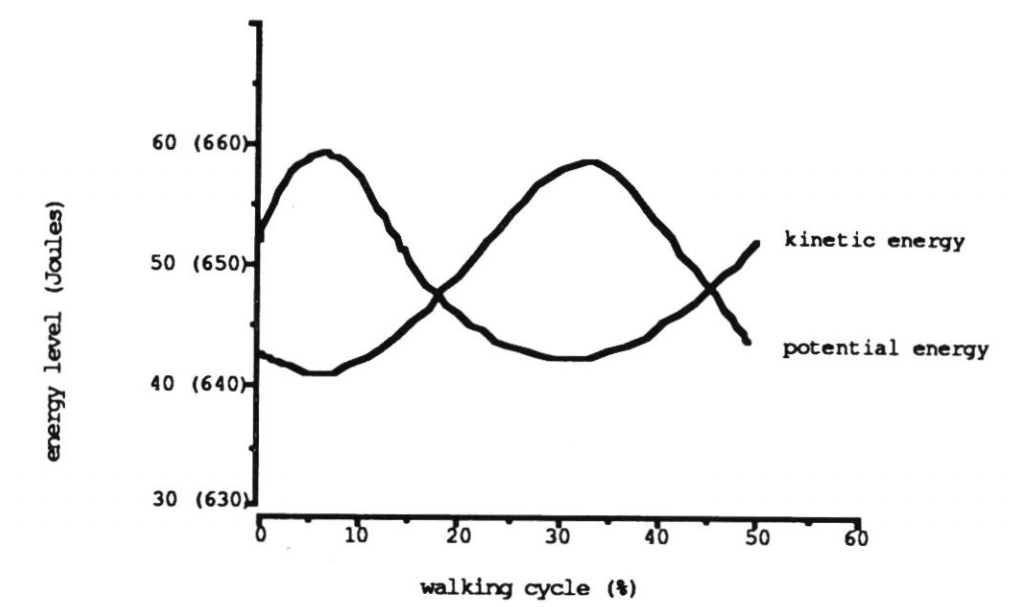
\includegraphics{fig/bruderlin.png}}
\caption{Aproximace kinetických a potenciálních energií horní poloviny těla pro průměrný krok. Převzato z \cite{bruderlin}.} \label{bruderlin_img}
\end{center}
\end{figure}

Tím je určen pohyb stojné nohy. Dále se určí rotace, úklon a náklon pánve. Rotace pánve je na maximu při úderu paty na zem a na minimu v mezistoji. Úklon pánve má minimum při úderu paty a maximum na konci dvojí opory. Náklon pánve je způsobem tím, že se tělo vždy nakloní na stranu nohy nesoucí váhu. Je minimální při úderu paty a maximální uprostřed stojné fáze. Pozice kyčle nohy ve švihu je určena interpolací těchto hodnot. Pohyb nohy ve švihu je rozdělen do tří fází a určen lineární interpolací. Pohyb horní poloviny těla je určen v závislosti na spodní, např. ruka se hýbe dopředu s protilehlou nohou. Pohyb ruky a rotace ramene je určen nastavitelnými atributy.

\section{Animation of Human Walking in Virtual Environments}
Kontrolní systém pro animaci lidské chůze po nerovném terénu je prezentován v článku Animation of Human Walking in Virtual Environments \cite{chung}. Používá se model člověka s 18 klouby a celkem 36 stupni volnosti. 

Kontrola pohybu na nejvyšší úrovni umožňuje uživateli animovat pohyby s malým množstvím parametrů. Uživatel specifikuje cestu pohybu pomocí kubických splinů v horizontální rovině. Z parametrů výšky člověka a rychlosti chůze je vygenerována délka a frekvence kroku. Pro normální chůzi může být vztah určen jako v rovnici:
\begin{eqnarray}
l &=& \sqrt{0.004 \times s \times h}\label{r.step_length}
\end{eqnarray}
kde $l$ je délka kroku, $s$ je rychlost trupu a $h$ je výška člověka.
Výpočet pozice chodidla na~terénu je určen jako funkce délky kroku, změny směru globální cesty a stavu terénu. Prvně jsou pozice chodidel rovnoměrně rozloženy po křivce cesty v horizontální rovině. Jestliže přesáhne rotace chodidla prahovou hodnotu, je krok zkrácen, ale doba provedení kroku zůstane zachována. Stav terénů ve 3D je zkontrolován pro určení bezkolizních trajektorií nohou. 

Na střední úrovni kontroly jsou poskytnuty atributy pro kontrolu spodní části těla. Prvně se odhadnou úhly dopadu a zvednutí chodidla stojící nohy. Z těchto odhadnutých hodnot a podle přibližné trajektorie pánve jsou pomocí inverzí kinematiky dopočítány úhly kolene a kyčle. Poté jsou přesně dopočítány úhly dopadu a zvednutí chodidla. Trajektorie chodidla se určí lineární interpolací mezi položeným chodidlem na zemi a úhly dopadu a~zvednutí chodidla. Tím je určena trajektorie stojící nohy, jednoho z koncových efektorů pro řetězec inverzní kinematiky. Nyní je potřeba určit pohyb kořene řetězce, pánve. 

Observace ukázaly, že trajektorie pánve přibližně odpovídá sinusoidě, viz obrázek \ref{chung_pelvis}. Pro interpolaci jsou použity kubické spliny, konkrétně Beziérova křivka. Pánev prochází vertikálním maximem uprostřed stojné fáze, tato hodnota se určí podle velikosti ohybu kolene. Pánev prochází minimem uprostřed intervalu dvojí opory, kdy obě nohy jsou v kontaktu se zemí. Pozice v této fázi je určena tak, aby byla minimalizována suma úhlových zrychlení všech kloubů podpírající nohy. Uživatel může těmto kloubům nastavovat váhy. Výsledná Beziérova křivka je poté nerovnoměrně vzorkována, aby bylo dosaženo nejrychlejšího pohybu během dvojí opory a nejpomalejšího uprostřed stojné fáze. 
\begin{figure}[h]
\begin{center}
\scalebox{0.4}{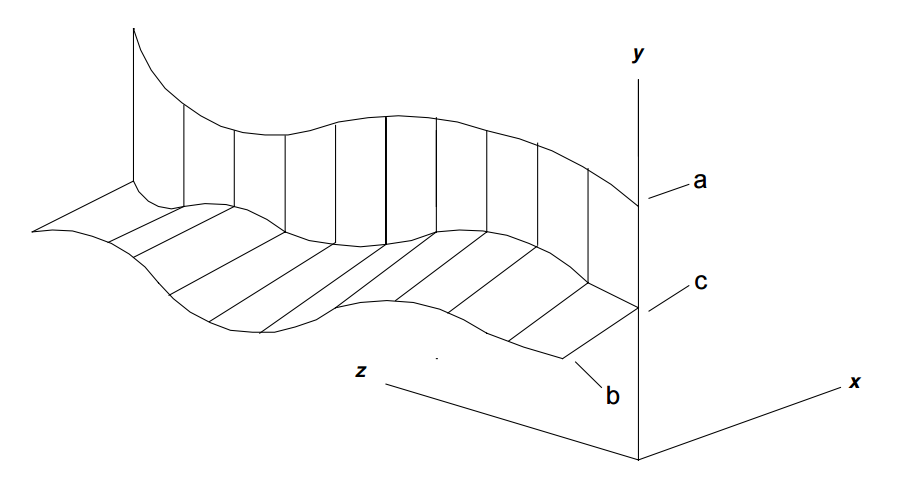
\includegraphics{fig/chung_pelvis.png}}
\caption{3D trajektorie (c) je určena z vertikálního (a) a horizontálního (b) posuvu. Převzato z \cite{chung}.} \label{chung_pelvis}
\end{center}
\end{figure}
Pro definici trajektorie chodidla nohy ve švihové fázi se použijí Beziérovy křivky obdobně jako při pohybu pánve. Spolu se znalostí pozice kořene kinematického řetězce (pánve) se dopočítají pozice ostatních kloubů. Trajektorie se určí tak, aby se chodidlo vyhnulo kolizím a aby byla spotřebována co nejmenší energie. Na nejnižší úrovni je poté možné nastavit další atributy (např. rotace a náklon pánve).

\chapter{Návrh a realizace řešení}
Řešení je implementováno v jazyce C++. 3D grafika je vykreslena pomocí rozhraní OpenGL. OpenGL je multiplatformní rozhraní, podporované množstvím programovacích jazyků, které umožňuje vykreslování 2D a 3D grafiky. Komunikuje s grafickým procesorem pro hardwarově akcelerované vykreslování. Pro zpracování vstupů a vytvoření kontextu OpenGL je využita knihovna SDL 2.0. SDL je multiplatformní knihovna umožňující nízkoúrovňový přístup ke klávesnici, myši, zvuku a grafickému hardwaru. Funguje nativně v C++.

Aplikace bude umožňovat načtení předpřipraveného modelu s připojenou kostrou. Případně uživatel může využít poskytnutou předpřipravenou kostru a na ní připojit vlastní model a ten poté vyexportovat v Blenderu do formátu \textit{COLLADA}. Aplikace model zobrazí za využití Linear blend skinning (kapitola \ref{linear_blend_skinning}) algoritmu. Uživatel bude mít možnost zobrazení pouze kůže modelu, nebo kostry, nebo obojího zároveň. Model bude rozhýbán animací chůze. Bude možné upravit animaci pomocí parametrů. K tomu bude využito grafické uživatelské rozhraní. Animace bude schopna se přizpůsobit nerovnému terénu.

\section{Načtení modelu}
Model je načítán z formátu COLLADA \cite{collada}, který podporuje uložení geometrie, efektů, fyziky, animace, kinematik scény aj. Využívá XML schéma. Při načítání uvažujeme, že~model do tohoto formátu byl exportován z Blenderu.

Začne se načtením geometrie modelu z XML elementu  \texttt{library\_geometries}. Uloží se pole s pozicemi vrcholů, normálami a texturovacími koordináty. Načtou se seznamy polygonů, které jsou určeny odkazy do polí načtených v předchozím kroku. Očekává se použití pouze trojúhelníků. Těchto seznamů může být více, liší se použitým materiálem a~v~naší aplikaci jeden tento seznam tvoří jeden  \textit{Mesh} (kód \ref{weighted_mesh}). Název materiálu je nastavený v~Blenderu a při načítání modelu se očekává přiložení textury ve formátu png se shodným názvem a příponou \texttt{\_D} pro difuzní texturu.

\begin{lstlisting}[float,floatplacement=H,language=C++, caption={Třída modelu.}, label={weighted_mesh}]
class Mesh {
protected:
  std::vector<glm::vec3> v; //pozice vrcholu
  std::vector<glm::vec3> n; //normaly
  std::vector<glm::vec2> t; //texturovaci koordinaty
  std::shared_ptr<Material> m; //material
public:
  /* ... */ };
  
class WeightedMesh : public Mesh {
private:
  std::vector<glm::vec4> weights; //vahy prirazenych kosti
  std::vector<glm::ivec4> jointIndices; //prirazene kosti
public:
  /* ... */ };
\end{lstlisting}

Následuje načtení vah a přiřazení kostí vrcholům z elementu  \texttt{library\_controllers}. První se přečte \textit{bind shape} matice. Ta popisuje transformaci geometrie do správného souřadného systému pro použití s klouby. Poté je načten seznam názvů kostí, seznam inverzních bind pose matic $\mathbf{B}_i$ (viz rovnice \ref{r.transform_mat}) pro každou kost a seznam vah vrcholů. Následuje seznam, který určuje pro každý vrchol počet kostí, které ho ovlivňují a stejný počet odkazů do seznamu kostí a vah.

Nyní se načte samotná hierarchie kostry z XML elementu \texttt{library\_visual\_scenes}. První uzel obsahuje kořenovou transformaci, od které se odvíjí další transformace všech kostí. Kosti jsou hierarchicky zanořené, obsahují název a lokální transformační matici, viz kód \ref{collada_skeleton}. Kosti se ukládají do 2D pole, kde každá kost má uložený index nadřazeného uzlu, tedy rodičovské kosti a $0 \dots n$ indexů na své potomky, viz kód \ref{class_skeleton}. Kostem se následně přiřadí inverzní bind pose matice vynásobené bind shape maticí, ta se dále neukládá. Pro~správné zobrazení kostry je nutné určit velikost kostí, ta se určí jako rozdíl pozice dané kosti a jejího potomka. Pokud ale kost nemá žádného potomka nemůžeme zjistit její velikost. Proto uvažujeme poloviční velikost než je velikost rodičovské kosti.

\begin{lstlisting}[float,floatplacement=H,language=C++, caption={Třída kostry.}, label={class_skeleton}
]
struct Bone {
  glm::mat4 localMat; //lokalni transformace
  glm::mat4 inverseBindMatrix; //inverzni bind pose matice
  int parent; //odkaz na rodicovskou kost
  std::vector<int> childs; //odkaz na potomky
  float scale; //velikost kosti, slouzi pro zobrazeni kosti 
};

class Skeleton {
private:
  std::vector<Bone> bones; //pole kosti
  glm::mat4 rootTransform; //korenova transformacni matice
  std::vector<glm::mat4> globalMat; //globalni transformace
public:
  /* ... */ };
\end{lstlisting}

Nakonec jsou naplněny objekty třídy \texttt{WeightedMesh} (kód \ref{weighted_mesh}). Abychom mohli použít \texttt{vec4} pro vstup kostí do vertex shaderu, musí mít každý vrchol přiřazené maximálně čtyři kosti. Pro model lidského těla jsou čtyři kosti dostatečné a pokud je jich více, mají některé velmi nízké váhy. Proto jsou pro každý vrchol seřazeny všechny jeho kosti sestupně podle vah a uloženy pouze první čtyři. Váhy ostatních jsou rozloženy rovnoměrně mezi ostatní, aby zůstala zachována podmínka o celkovém součtu všech vah (viz sekce \ref{weight_sum}).

\begin{lstlisting}[float,floatplacement=H,language=XML, caption={Ukázka uložení hierarchie kostry ve formátu COLLADA.}, label={collada_skeleton}]
<library_visual_scenes>
  <visual_scene id="Scene" name="Scene">
    <!-- ... -->
    <node id="metarig" name="metarig" type="NODE">
      <matrix sid="transform">1 0 0 0 0 1 0 0 0 0 1 0 0 0 0 1</matrix>
      <node id="hips" name="hips" sid="hips" type="JOINT">
        <matrix sid="transform">
          1 0 0 0 0 -0.16 -0.98 0.05 0 0.98 -0.167 1.01 0 0 0 1
        </matrix>
        <node id="spine" name="spine" sid="spine" type="JOINT">
          <matrix sid="transform">
            1 0 0 0 0 0.99 0.11 0.17 0 -0.11 0.99 1.49e-8 0 0 0 1
          </matrix>
          <node id="chest" name="chest" sid="chest" type="JOINT">
            <matrix sid="transform">
              1 0 0 0 0 0.99 0.14 0.15 0 -0.14 0.99 7.45e-9 0 0 0 1
            </matrix>
            <!-- ... -->
          </node>
        </node>
        <!-- ... -->
      </node>
    </node>
    <!-- ... -->
  </visual_scene>
</library_visual_scenes>
\end{lstlisting}

\section{Zobrazení}
Před každým zobrazením snímku je nutné spočítat globální transformační matice pro všechny kosti kostry. Proto procházíme pole s kostmi a pro každou kost vynásobíme globální matici rodiče s její lokální maticí. Poté získáme transformační matici $\mathbf{T}$ podle rovnice \ref{r.transform_mat}. Následně nastavíme kořenovou transformační matici jako transformační matici modelu. Dále ve vertex shaderu získáme pozici vrcholu kůže násobením maticí $\mathbf{T}$ a odpovídající vahou pro čtyři přiřazené kosti. Přepočítáváme také normálu, viz kód \ref{animation_shader}.

\begin{lstlisting}[float,floatplacement=H,language=GLSL, caption={Ukázka z vertex shaderu pro animovaný model. Výpočet pro pozici a normálu se provede 4krát, pro komponenty \texttt{x}, \texttt{y}, \texttt{z} a \texttt{w} vektorů \texttt{v\_weights} a \texttt{v\_joints}.}, label={animation_shader}]
vec4 pos = vec4(0.0);
pos += T[v_joints.x] * vec4(v_pos, 1.0) * v_weights.x;
/* ... */
vec3 norm = vec3(0.0);
norm += ti_T[v_joints.x] * v_norm * v_weights.x;
/* ... */
gl_Position = mvp * vec4(pos.xyz, 1.0);
\end{lstlisting}

Následuje zobrazení kostry. Pro každou kost se použije shodný model. Pro kosti se používají globální matice shodné jako při zobrazování kůže, ale je v nich započítané zvětšení, aby na sebe kosti navazovaly.  Výsledná transformační matice kosti je kořenová transformace vynásobená s touto globální maticí kosti. Před zobrazením je vyčištěn hloubkový buffer, aby se kostra překreslila přes kůži. Pro zobrazení jsou použity difuzní textury a Phongův osvětlovací model. Výsledný výstup je na obrázku \ref{graphical_output}.

\begin{figure}[h]
\begin{center}
\subfloat{{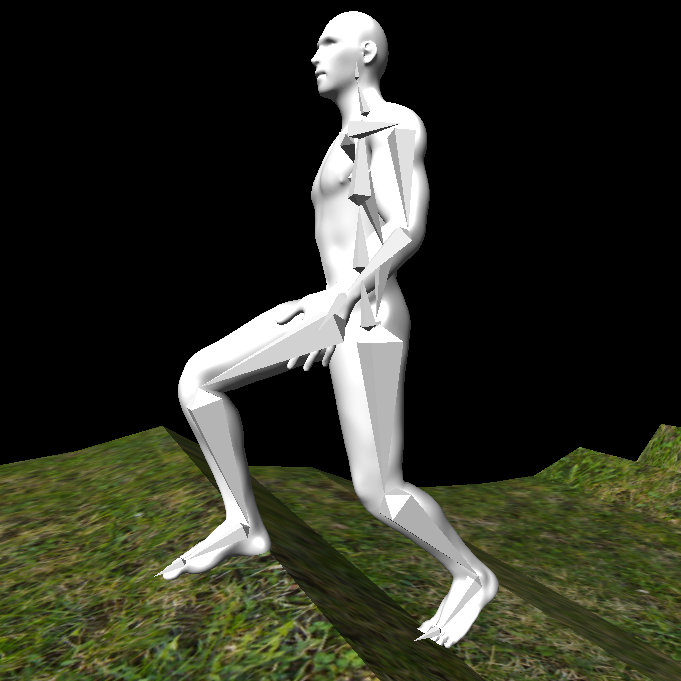
\includegraphics[width=7cm]{fig/teaser1.png}}}
\qquad
\subfloat{{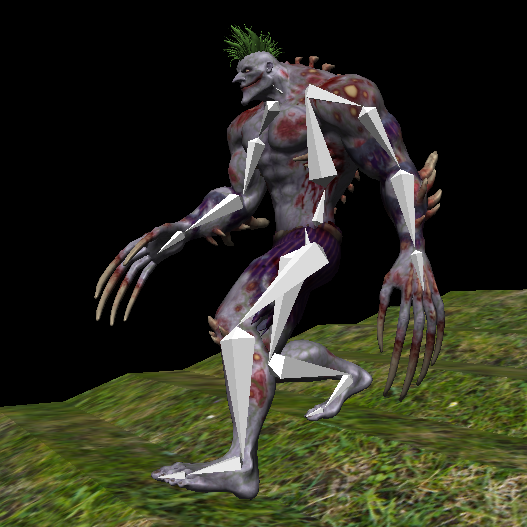
\includegraphics[width=7cm]{fig/teaser2.png}}}
\caption{Grafický výstup aplikace pro dva různé modely. Model vlevo je převzat z \cite{male_mesh} a vpravo z \cite{venom}.} \label{graphical_output}
\end{center}
\end{figure}

\subsection{Terén}
Jako terén pro demonstraci animace se využívá \textit{výškové pole}. Výškové pole se skládá ze~čtverců spojených v jedné řadě, jejichž spojné úsečky mohou mít různou výšku. Terén může mít tři varianty. Buď je celý rovný, nebo má schodovitý tvar a nebo je náhodně vygenerovaný. 

Pro náhodně vygenerovaný terén je použit \textit{Midpoint} algoritmus v jedné dimenzi \cite{midPoint}. Algoritmus začíná s jednou horizontální úsečkou. Opakovaně nalezne prostřední bod úsečky a změní jeho výškovou souřadnici o náhodnou hodnotu a přitom sníží rozsah této náhodné hodnoty pro další použití. Algoritmus je implementovaný rekurzivně. To jak bude terén hladký nebo naopak hrubý je určeno konstantou $0.0 \leq \mathbf{H} \leq 1.0$. Rozsah náhodné hodnoty je pro každé zanoření vynásoben $2^{-\mathbf{H}}$, tzn. pro velké hodnoty $\mathbf{H}$ bude terén velmi hladký a pro malé $\mathbf{H}$ bude zase velmi hrubý, viz obrázek \ref{terrain}. 

\begin{figure}[h]
\begin{center}
\subfloat{{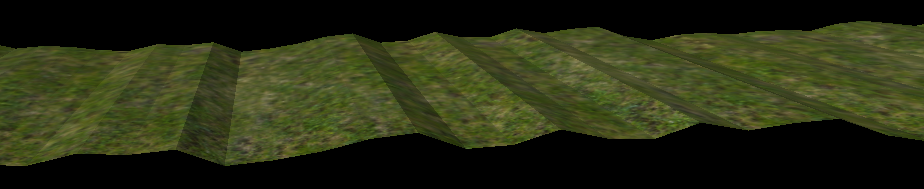
\includegraphics[width=13cm]{fig/midPoint_03.png}}}
\qquad
\subfloat{{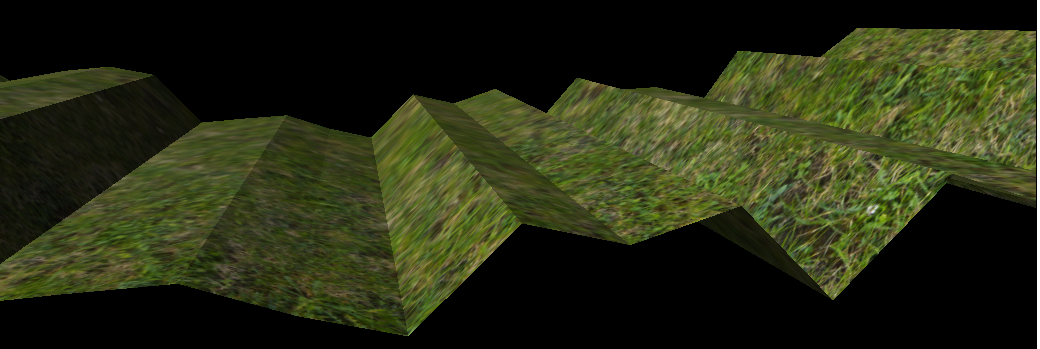
\includegraphics[width=13cm]{fig/midPoint_01.png}}}
\caption{Terén vygenerovaný pomocí Midpoint algoritmu -- nahoře pro $\mathbf{H} = 0.3$ a dole pro $\mathbf{H} = 0.1$.} \label{terrain}
\end{center}
\end{figure} 

\section{Animace}
Animace je vytvářena nad kostrou z obrázku \ref{bone_structure}, tedy model musí mít připojenou právě tuto kostru, aby animace fungovala. Popis animace je rozdělen na pohyb nohou, pánve a~horní poloviny těla. Ve všech těchto částech je potřeba určovat rotace a trajektorie kloubů. K~tomu slouží Bézierovy křivky. Prvně je určen pohyb pánve a poté se za využití inverzní kinematiky nastaví klouby nohou. Horní končetiny se hýbou opačně k dolním končetinám. Při popisu animace budeme využívat referenčních rovin zobrazených na obrázku \ref{fig:ref_planes}.

\begin{figure}[h]
	\centering
	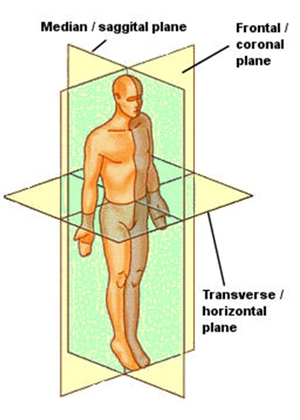
\includegraphics[width=0.35\linewidth]{fig/ref_planes.jpg}
	\caption{Referenční roviny pohybu -- horizontální, frontální a sagitální.\protect\footnotemark}
	\label{fig:ref_planes}
\end{figure}

\subsection{Bézierovy křivky}
\textit{Bézierovy křivky} \cite{bezier_primer} jsou parametrické interpolační křivky, které nám umožní přesnou aproximaci s malým množstvím kontrolních bodů. Zvolili jsme kubické Bézierovy křivky, které používají čtyři kontrolní body, kde křivka prochází pouze krajními. Dva prostřední body určují tvar křivky. Segmenty těchto křivek je možné skládat za sebe. Jestliže chceme plynulou návaznost, je nutné zajistit aby třetí bod předchozího segmentu a druhý následujícího byly kolineární. Máme-li parametr $t$ potom se pozice $\mathbf{B}$ na křivce určí následovně:
\begin{eqnarray}
\mathbf{B}(t) &=& (1 - t)^3\mathbf{P_0} + 3(1-t)^2 t\mathbf{P_1} + 3(1-t)t^2\mathbf{P_2} + t^3\mathbf{P_3}
\label{r.bezier}
\end{eqnarray}
kde $0 \leq t \leq 1$ a $\mathbf{P_0}$, $\mathbf{P_1}$, $\mathbf{P_2}$ a $\mathbf{P_3}$ jsou kontrolní body křivky.

Křivky, které chceme aproximovat jsou ve 2D prostoru. Potřebujeme pro konkrétní hodnotu $x$ získat odpovídající hodnotu $y$. Bézierovy křivky ale vrací hodnotu podle parametru $t$, který se nepohybuje po křivce lineárně. Proto musíme pro naše $x$ určit odpovídající $t$ a~to poté použít pro získání $y$. To je možné řešit tak, že se určí větší množství bodů na křivce (např. 100) a pro každý se získá hodnota $x$. Když je potom potřeba určit $t$ pro nějaké $x$, najde se vhodný interval a $t$ se určí lineární interpolací. Protože se ale naše křivky budou měnit s nastavováním parametrů a nerovností terénu, toto řešení není vhodné, protože vyžaduje při každé změně přepočítat všechny hodnoty. Proto jsme zvolili řešení numerickou metodou.

Zvolili jsme metodu Regula Falsi, která slouží pro řešení jedné nelineární rovnice. Ta konverguje vždy a v našem případě kdy řeší hladké a monotónní křivky i velmi rychle. Funguje na principu dělení intervalu $\langle a, b \rangle$ na dvě obecně různé části. Dělícím bodem intervalu je průsečík osy $\mathbf{x}$ s úsečkou spojující $[a,f(a)]$ a $[b,f(b)]$ určený následovně:
\begin{eqnarray}
x_k &=& b_k - \frac{b_k-a_k}{f(b_k)-f(a_k)}f(b_k)
\label{r.regula_falsi}
\end{eqnarray}
Výpočet končí jestliže $|x_k - x_{k-1}| < \epsilon$. Tato metoda najde v našem případě odpovídající parametr $t$ s dostatečnou přesností na cca 4 iterace.

\footnotetext{Převzato z \url{http://sme-chinoises-euronext.typepad.fr/artbot/2014/09/a-study-of-walking-in-order-to-design-a-biped-robot.html}}

\subsection{Pohyb nohou}
O pohyb nohou se stará třída \texttt{Leg}, jejíž hlavní metodou, která se volá každý snímek poté co je již pohnutá pánev je metoda \texttt{update}. Ta využívá jediný parametr a tím je čas, o který se animace posunula. Jeden krokový cyklus nohy je nastaven na dobu trvání jedné vteřiny. Zrychlení nebo zpomalení kroku je dosaženo úpravou vstupního času. Tento vstupní čas je poté přičten k proměnné \texttt{t}, která se při přetečení přes 1 vteřinu vrací o vteřinu zpět. Podle \texttt{t} se poté určí v jaké fázi krokového cyklu se noha nachází a podle toho je určen další postup.

Nemusíme rozlišovat všech sedm fází cyklu, ale budou nám stačit čtyři. Stádium zatěžovaní a mezistoj jsou nezměněny. Konečný stoj a předšvihová fáze jsou spojeny do jedné, protože z pohledu animace se tyto fáze neliší, v obou je prováděn stejný úkon -- zvedání paty. Poslední tři fáze (počáteční švih, mezišvih a konečný švih) jsou také spojeny do jedné, budeme ji říkat pouze švihová. Tyto fáze je možné spojit, protože celá švihová fáze může být popsána spojitě pomocí trajektorie od odrazu palce do počátečního kontaktu.

Pro potřeby správného a přesného určování pohybu nohou potřebujeme znát pozici paty a prstů nohy. Přesně se tyto pozice nedají získat pouze z pozic kostí. Tyto pozice jsou závislé na pozici a rotaci chodidla. Jsou určeny podle umístění kostry v prostoru před samotným provedením animace, viz obrázek \ref{fig:pozice_paty}. Takto získané pozice paty a prstů nohy jsou vynásobeny inverzní transformační maticí chodidla. Tím jsou získány relativní pozice vůči chodidlu, z kterých je později možné získat přesně pozici paty a prstů v závislosti na aktuální pozici a rotaci chodila. Stačí vynásobit aktuální transformační maticí chodidla a~tyto relativní pozice.

\begin{figure}[h]
	\centering
	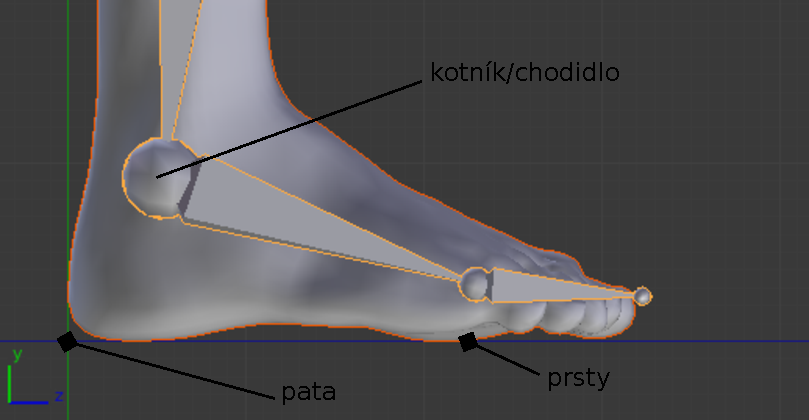
\includegraphics[width=0.7\linewidth]{fig/pozice_paty.pdf}
	\caption{Vstupní pozice modelu a jeho kostry. Pozice paty má shodné $x$ s kotníkem, ale nulové souřadnice na ose $\mathbf{z}$ a $\mathbf{y}$. Pozice prstů nohy má nulovou souřadnici na ose $\mathbf{y}$.}
	\label{fig:pozice_paty}
\end{figure}

Důležitou podmínkou pro chůzi po nerovném terénu je možnost získat informace o~terénu, na kterém se noha nachází. Terén je objekt, který je sdílený všemi součástmi těla, které s~ním potřebují pracovat. Pro nohu je důležité získat výšku terénu pod patou nohy a~úhel mezi chodidlem a~terénem. Tento úhel se určí pomocí skalárního součinu mezi vektorem směřujícím od paty k prstům nohy a~vektorem mezi pozicemi na terénu pod patou a pod prsty. 

\subsubsection{Stádium zatěžování}
Stádium zatěžování nastane pro $t < 0.12$. Před prvním vykonáním této fáze se dokončí švihová fáze. Protože předchozí snímek se vykonával pro nějaké $t < 1.0$ a v aktuálním snímku se přesunul z švihové fáze do stadia zatěžování s nějakým $t >= 0.0$ je potřeba prvně dokončit předchozí fázi jako by čas byl roven 1. Kdybychom to neudělali animace by nebyla plynulá, jak moc by záviselo na velikosti časového kroku. Také je získán počáteční úhel mezi chodidlem a terénem. 

Tato fáze se zabývá zachováním pozice paty na terénu a sklápěním chodidla. Pánev se v každém snímku pohne první, proto je noha na jiné pozici než byla v předchozím snímku. Rotace chodidla se v této fázi určuje lineární interpolací mezi počátečním úhlem s~terénem a nulovým úhlem. Protože je pozice paty závislá na rotaci chodidla, musíme prvně natočit chodidlo do požadovaného úhlu se zemí pro aktuální \texttt{t}. Nyní se může určit rozdíl mezi aktuální pozicí paty a předchozí. Z toho určit požadovanou pozici kotníku a~pomocí inverzní kinematiky kotník do této pozice nastavit. Inverzní kinematika hýbe nohou a tím i~mění rotaci chodidla vůči terénu. Proto je po jejím provedení potřeba znovu natočit chodidlo do správného úhlu.

\subsubsection{Mezistoj}
Následující fáze mezistoj nastává pro $0.1 \leq t < 0.31$ a má za úkol udržet chodilo položeno na~zemi na stejné pozici. Je vykonávána podobně jako předchozí fáze. Před prvním vykonáním je tedy prvně dokončeno stádium zatěžování. Rozdílem je, že pohyb nevychází z paty, ale vychází z kotníku. Proto nám stačí si na začátku zapamatovat pozici kotníku a tu použít pro inverzní kinematiku. Není tedy před jejím provedením nutné nastavovat novou rotaci chodidla pro určení pozice paty. Rotace je nastavena až po provedení inverzní kinematiky tak, aby úhel mezi terénem byl nulový.

\subsubsection{Zvedání paty}
Zvedání paty nastává pro $0.31 \leq t < 0.62$. Pro čas do $t = 0.5$ při zvedání paty zůstává koleno převážně propnuté, ve zbylém čase se koleno ohýbá. Aby tohoto bylo dosaženo, není vhodné zvedat patu v celé fázi lineárně. Také není vhodné ji rozdělit na dvě samostatné části, potom by zvedání paty nepůsobilo plynule. Nejvhodnějším řešení se zdá použití Bézierovy křivky, kde v první části se zvedá pata méně a v druhé více a celá fáze je plynulá. Konkrétní tvar křivky (obrázek \ref{fig:heelRiseRot}) byl určen experimentálně tak aby tato fáze byla dostatečně přirozená. Také je u této křivky důležitý sklon u konce fáze, který při vhodném zvolení zajistí co~nejplynulejší přechod do švihové fáze, tzn. je důležité aby rychlost pohybu paty na konci této fáze a na začátku švihové byly co nejpodobnější. Rychlost pohybu nohy ve švihové fázi je závislá na délce kroku. Proto je celkový úhel, o který je pata zvednutá, zvětšován se zvětšující se délkou kroku. Mimo správnou návaznost je toto zvětšování také nutné pro~zvýšení efektivního dosahu nohy, aby byl vůbec delší krok umožněn. Křivka úhlu zvedání paty je vytvořena pro~nejdelší možný dvojkrok, který je 1.8 metru dlouhý. Pro jiné délky kroku je vynásobena $c = (dvojkrok/1.8)^2$, tato hodnota byla také zjištěna experimentálně, aby tato fáze vypadala přirozeně.

\begin{figure}[h]
	\centering
	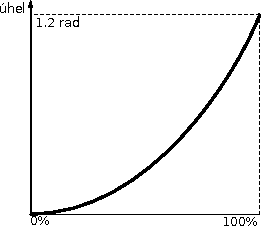
\includegraphics[width=0.3\linewidth]{fig/heelRiseRot.pdf}
	\caption{Rotace  chodidla vůči zemi při fázi zvedání paty pro délku dvojkroku 1.8 metru.}
	\label{fig:heelRiseRot}
\end{figure}

Samotné zvedání paty probíhá následovně. Na začátku fáze se uloží pozice prstů, která se bude udržovat. Následně se chodidlo nastaví do úhlu se zemí určeného z křivky zvedání paty. Dále se může určit pozice prstů nohy a posunout kotník o rozdíl původní a aktuální pozice prstů. Tím se kotník dostane do požadované polohy, ale prsty v původní pozici nebudou, protože inverzní kinematika změnila rotaci chodidla vůči zemi. Proto je chodidlo znovu natočeno na správný úhel. Nakonec zbývá jenom natočit prsty nohy, aby byly v~nulovém úhlu se zemí, tzn. natočit na rotaci odpovídající úhlu mezi chodidlem a zemí.

\subsubsection{Švihová fáze}
Švihová fáze nastává pro $0.62 \leq t \leq 1.0$. Jejím cílem je přesunutí nohy z aktuální pozice na~pozici dalšího kroku. V této fázi se využívají čtyři Bézierovy křivky. Při prvním vykonání této fáze se dokončí fáze zvedání paty a zapamatuje se pozice paty, která bude sloužit jako výchozí bod pro švihovou fázi. V průběhu této fáze je také potřeba vrátit prsty na noze do původní polohy, protože při zvedání paty byly otočeny. V první pětině švihové fáze jsou prsty rotovány do pozice určené lineární interpolací mezi otočenou pozicí a původní nataženou pozicí.

Podle \cite{chung} se chodidlo pohybuje vpřed s měnící se rychlostí.  Rychlost je nejvyšší uprostřed švihové fáze a nejpomalejší na začátku a na konci. K tomu slouží Bézierova křivka určující posun chodidla v horizontální rovině, viz obrázek \ref{fig:swingSpeed}. Tato křivka je vytvořena pro posun o délce 1 metr. Potom pro různé délky stačí před použitím křivky její kontrolní body vynásobit požadovanou délkou. Jako délku nemůžeme použít aktuální délku dvojkroku, to by se noha přesouvala před požadovanou pozici. Je nutné vzít v úvahu, že při zvedání paty se již  pata posunuje vpřed. Noha zná pozici paty na začátku aktuálního kroku a pozici, na kterou chceme aby pata dopadla na konci kroku, tedy začátku dalšího. Pata zůstává na stejné pozici při stádiu zatěžování a při mezistoji. Ale při zvedání paty se již pohybuje v~horizontální rovině. Délka tohoto pohybu se musí odečíst od délky dvojkroku, abychom získali přesný zbývající posun nohy na cílovou pozici pro vynásobení Bézierovy křivky. Pro posun vpřed v horizontální rovině poté stačí zjistit hodnotu křivky a přičíst ji k pozici po~ukončení zvedání paty.

\begin{figure}[h]
	\centering
	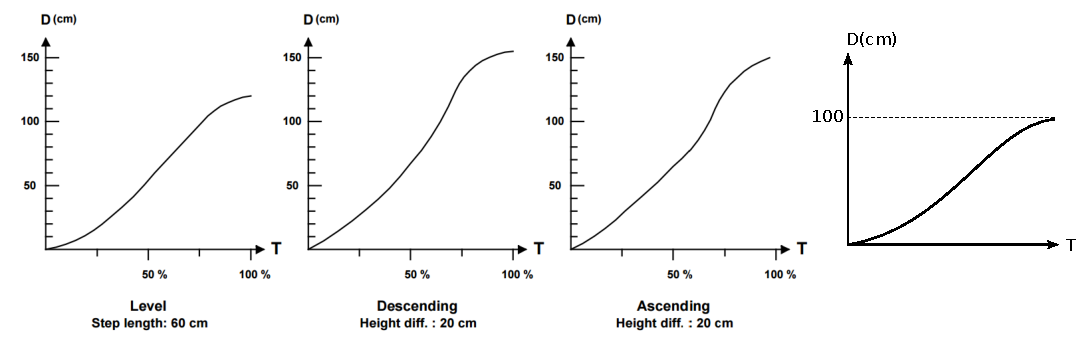
\includegraphics[width=1.0\linewidth]{fig/leg_swing_speed.pdf}
	\caption{Vlevo jsou naměřené grafy posunu chodidla v čase pro chůzi po rovině, z kopce a do kopce převzaté z článku \cite{chung}. Vpravo je vytvořená generická Bézierova křivka, která je použita pro posun nohy v horizontální rovině.}
	\label{fig:swingSpeed}
\end{figure}

V průběhu chůze může být nastavena různá šířka kroku. Není přirozené, aby si chodidlo v průběhu celé švihové fáze udržovalo stejnou vzdálenost do šířky od pánve. Působí mnohem věrohodněji, pokud se chodidlo po odrazu od země přesune na šířku kyčle, které dosáhne v polovině švihové fáze, a poté se začne přesouvat zpět na šířku kroku, které dosáhne v~okamžiku dopadu paty. To by bylo možné vyřešit lineární interpolací mezi šířkou kroku a~pozicí kyčle. Tímto způsobem ale animace není plynulá kvůli náhlému zrychlení nohy při odrazu paty a zastavení při dopadu. Proto jsme vytvořili další Bézierovu křivku, která se použije pro plynulé zrychlení a zpomalení tohoto pohybu, viz obrázek \ref{fig:widthStep}. Časový parametr lineární interpolace se použije pro získání hodnoty této křivky, která se použije místo něho.

\begin{figure}[h]
	\centering
	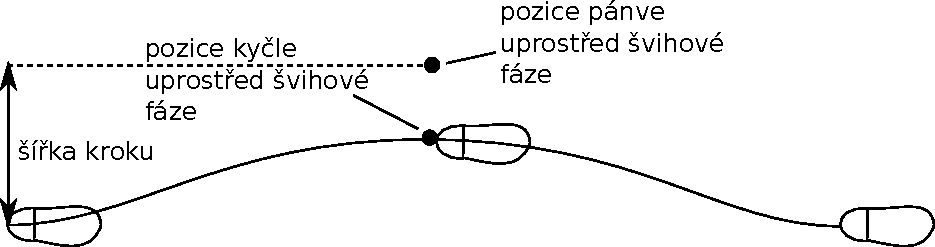
\includegraphics[width=0.7\linewidth]{fig/svih_sirka_kroku.pdf}
	\caption{Přesun chodidla během švihové fáze v závislosti na šířce kroku.}
	\label{fig:widthStep}
\end{figure}

Takto jsou získány dva údaje ze čtyř, které jsou potřeba pro určení pozice chodidla ve~švihové fázi. Máme pozici paty do šířky, vpřed a dále potřebujeme výšku a rotaci chodidla. Až budeme mít všechny tyto čtyři údaje, můžeme nastavit správnou rotaci v kotníku. A~poté z~ní určit novou pozici kotníku tak, aby pata byla na správné pozici podle naší určené šířky, výšky a posunu vpřed. S touto novou pozicí kotníku se spočítá inverzní kinematika. Zbylé dva údaje rotace a výšky chodidla je prvně nutné přizpůsobit nerovnému terénu.

Pro rotaci chodidla v průběhu švihové fáze vycházíme z obrázku \ref{fig:ankleRot}, kde je uvedena rotace v kotníku v průběhu celého cyklu. Část toho grafu ve švihové fázi je aproximována pomocí Bézierovy křivky. Tato křivka začíná pro 15 stupňů plantární flexe, tedy propnutí kotníku z neutrální polohy, a končí u přibližně neutrální polohy. Tuto křivku je nutné přizpůsobit propnutí kotníku na začátku švihové fáze, které se může lišit v závislosti na~délce kroku a sklonu terénu. Kontrolní body křivky jsou proto vynásobeny koeficientem $c = aktRot / 15\degree$, kde $aktRot$ je aktuální propnutí v kotníku. 

\begin{figure}[h]
	\centering
	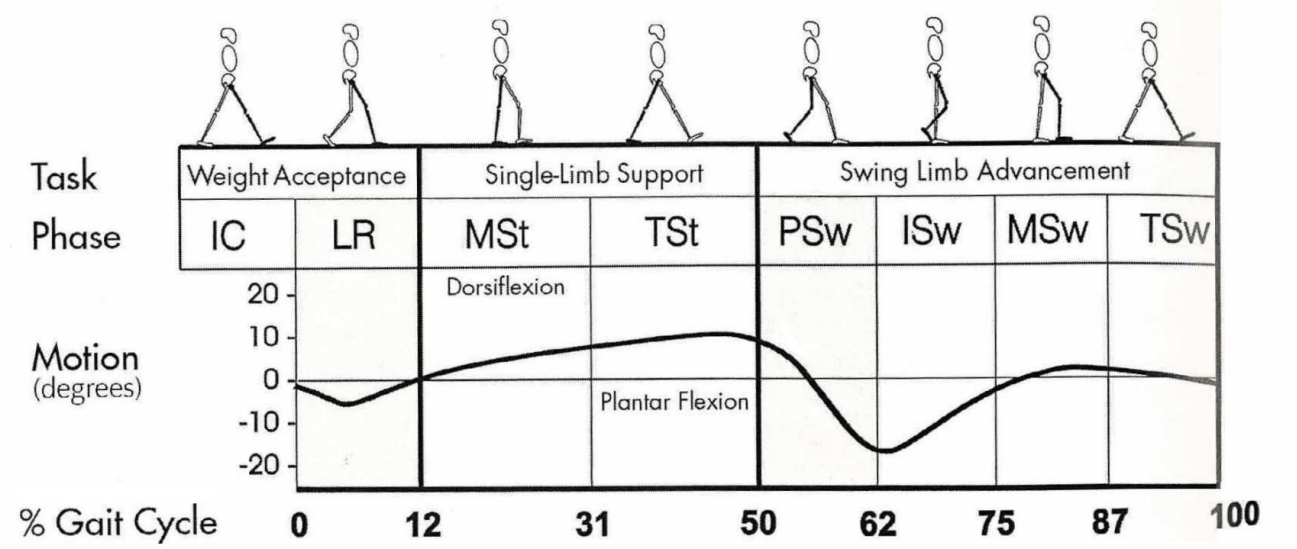
\includegraphics[width=0.9\linewidth]{fig/ankle_kinematics.png}
	\caption{Rotace kotníku v průběhu krokového cyklu. Převzato z \cite{biomechanika_chuze}.}
	\label{fig:ankleRot}
\end{figure}

Nyní je potřeba vyřešit úhel dopadu chodidla na terén. Jedna možnost je mít pevně daný úhel, pod kterým bude chodidlo vždy dopadat. Zdá se ale přirozenější, nechat úhel podle naší křivky a upravit ho jenom v nevhodných případech. Tímto případem je možnost průchodu chodidla skrz terén při sklonu do kopce (obrázek \ref{fig:swingRotFix}), ve kterém je rotace upravena tak, aby při dopadu byl sklon chodidla shodný s terénem. 

\begin{figure}[h]
	\centering
	
\includegraphics[width=0.6\linewidth]{fig/foot_through_terrain.pdf}
	\caption{Pozice chodidla na terénu při dopadu paty s původní rotací a po úpravě rotace.}
	\label{fig:swingRotFix}
\end{figure}

Pro úpravu rotace chodidla je nutné před samotným provedením kroku vyzkoušet pozici na konci kroku při dopadu paty. To vyžaduje určení transformační matice pánve při dopadu paty a posunutí nohy na cílovou pozici pomocí inverzní kinematiky. Poté je zkontrolován úhel mezi chodidlem a terénem. Jestliže je záporný, tzn. chodidlo se nachází pod terénem, je upravena křivka rotace. Potřebujeme upravit pouze koncový úhel propnutí kotníku, proto jsou o potřebný úhel posunuty poslední dva kontrolní body křivky.

Poslední co je potřeba určit je výška chodidla. K tomu slouží poslední Bézierova křivka použitá pro pohyb nohy, která je aproximována podle \cite{DadashiMarianiRochatEtAl2014}, viz obrázek \ref{fig:swingHeight}. Tato křivka určuje výšku paty a skládá se ze tří segmentů, to nám umožňuje křivku dobře tvarovat při přizpůsobování se nerovnému terénu. Obdobně jako při rotaci chodidla je tato křivka vytvořena pro jeden případ a poté upravena. Konkrétně je vytvořena pro patu nacházející se 20 centimetrů nad terénem při počátku švihové fáze. Pro případy, kdy se pata nachází výše nebo níže, jsou všechny kontrolní body vynásobeny koeficientem. Koeficient zajistí, aby výška paty odpovídala a švihová fáze plynule navazovala na zvedání paty.

\begin{figure}[h]
	\centering
	
\includegraphics[width=0.5\linewidth]{fig/legSwingCurve_excel.pdf}
	\caption{Výška paty při švihové fázi pro chůzi po rovném terénu.}
	\label{fig:swingHeight}
\end{figure}

Kvůli přizpůsobení křivky terénu se před samotným provedením kroku krok odsimuluje. K tomu je potřeba zvolit vhodný časový rozestup. Zvolili jsme, že se výpočet provede 50krát, to je dostatečně přesné i rychlé. V každém kroku simulace se určí pozice pánve a~pomocí inverzní kinematiky se noha přesune na novou pozici obdobným způsobem jako při samotném provádění kroku chůze. Poté se zkontroluje zda požadovaná pozice, určená mimo jiné právě křivkou výšky paty, byla v dosahu nohy, tzn. vzdálenost od kyčle k požadované pozici je větší než délka stehenní a holenní kosti. Jestliže není, je křivka v daném místě zvednuta. Poté, co je již pozice v dosahu, je zkontrolováno, zda se pata nebo prsty nohy nenachází pod~úrovní terénu. Jestliže ano, je křivka znovu adekvátně zvednuta. Tím jeden krok simulace končí.

Před samotnou simulací je křivka upravena tak, aby výška, tedy souřadnice na ose $\mathbf{y}$, posledního kontrolního bodu byla posunuta o $h$, kde $h$ je rozdíl výšky terénu aktuálního a~následujícího kroku. Toho je dosaženo vynásobením souřadnice $y$ koeficientem $c = x \times h$, kde $x$ je souřadnice na ose $\mathbf{x}$ a nabývá hodnot od 0 do 1. Tím je křivka přizpůsobena změně výšky terénu, je zachován její tvar a i plynulost díky zachování kolinearity kontrolních bodů při navazování segmentů. Další úprava křivky nastane, pokud při simulaci musí být křivka pro danou pozici na ose $\mathbf{x}$ zvednuta. Při této úpravě se prvně nalezne segment, do kterého spadá $x$. Budou upravovány okrajové kontrolní body tohoto segmentu (pokud nejsou okrajové pro celou křivku) a k nim přilehlé kontrolní body. Celkem tedy budou upravovány tři nebo jeden kontrolní bod na každé straně segmentu. Těmto bodům je k~souřadnici $y$ přičtena hodnota určující o kolik je potřeba křivku zvednout. Jestliže se $x$ nachází v~prostředním resp. druhém segmentu, je hodnota rozložena na obě strany tak, že čím více vlevo je $x$, tím jsou více zvedány levé kontrolní body a čím více vpravo, tím jsou více zvedány pravé kontrolní body. Při této úpravě je také zachována plynulost křivky. Příklad upravené křivky je na obrázku \ref{fig:swingHeightAdjusted}.

\begin{figure}[h]
	\centering
	
\includegraphics[width=0.4\linewidth]{fig/swingHeightAdjusted.pdf}
	\caption{Křivka určující výšku paty při švihové fázi přizpůsobená nerovnému terénu.}
	\label{fig:swingHeightAdjusted}
\end{figure}

\subsubsection{Inverzní kinematika}
Kinematický řetězec, který potřebujeme řešit, obsahuje pouze dva klouby -- kyčel a koleno. Pro takový řetězec existuje rychlé analytické řešení. Pozici kyčle známe a požadovanou cílovou pozici koncového efektoru (kotníku) také. Kromě toho známe i~délku stehenní a~holenní kosti. Rotace kyčle a kolene se poté dopočítá jako úhly v trojúhelníku pomocí kosinové věty.

Tímto ještě není inverzní kinematika vyřešená, protože může být nekonečně mnoho řešení s různými rotacemi okolo osy mezi kyčlí a kotníkem, viz obrázek \ref{fig:analytical_IK}. Pomocí kosinové věty jsme pro stehenní kost určili úhel $\alpha_1$, který určuje rotaci mezi vektorem $\mathbf{a}$ a stehenní kostí $\mathbf{v}$. Abychom nastavili kost do správné pozice, je potřeba vektor $\mathbf{v}$ natočit do $\mathbf{a}$. K~tomu je sestavena transformační matice, jejímž vynásobením se $\mathbf{v}$ dostane do $\mathbf{a}$. Poté je již možné rotovat kyčel o úhel $\alpha_1$ a rotovat holeň do úhlu $\alpha_2$. 

K tomu abychom určili výslednou rotaci okolo vektoru $\mathbf{a}$ slouží referenční vektor \cite{analytic_IK}. Výsledné řešení se poté vybere takové, aby úhel $\delta$ mezi referenčním vektorem a stehenní kostí byl co nejmenší. Proto budeme rotovat vektor $\mathbf{v}$ o úhel $\theta$ do nového vektoru $\mathbf{v}'$. Minimalizace úhlu $\delta$ je ekvivalentní maximalizaci $\cos\delta$ (resp. $\mathbf{v}'\cdot \mathbf{k}$) a to nastane když je první derivace rovna nule:
\begin{eqnarray}
\frac{d}{d\theta}\mathbf{v}'\cdot \mathbf{k} &=& 0
\label{r.IK_derivation}
\end{eqnarray}
Po úpravě dostaneme:
\begin{eqnarray}
\theta = \tan^{-1}\frac{2 B}{C-A} &\vee & \theta = \pi + \tan^{-1}\frac{2 B}{C-A}
\label{r.IK_derivation2}
\end{eqnarray}
kde $A = (\mathbf{a}\cdot \mathbf{v})\mathbf{a} \cdot \mathbf{k} - ((\mathbf{a} \times \mathbf{v})\times \mathbf{a})\cdot \mathbf{k}$, $B = (\mathbf{a} \times \mathbf{v})\cdot \mathbf{k}$ a $C = \mathbf{v}\cdot \mathbf{k}$. Abychom určili, které ze dvou řešení maximalizuje $\cos\delta$ musíme určit druhou derivaci $\cos\delta$:
\begin{eqnarray}
\frac{d^2}{d\theta^2}\cos\delta &=& \frac{A-C}{2} \cos\theta - B\sin\theta
\label{r.IK_derivation3}
\end{eqnarray}
Úhel $\delta$ je minimální, když je druhá derivace menší než nula.

\begin{figure}[h]
	\centering
	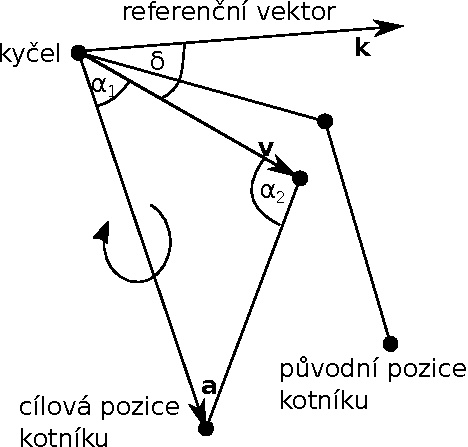
\includegraphics[width=0.4\linewidth]{fig/analytical_IK.pdf}
	\caption{Pro dosažení cílové pozice v kotníku se pomocí kosinové věty určí úhly v kyčli a v koleni. Rotace okolo osy mezi kyčlí a kotníkem se určí tak, aby úhel  $\delta$ byl co nejmenší.}
	\label{fig:analytical_IK}
\end{figure}

Referenční vektor směřuje vpřed ve směru chůze a leží v horizontální rovině. Důležité je, že tento vektor nevychází z kyčle, protože by byl ovlivněn rotacemi pánve v průběhu krokového cyklu a nohy by se vytáčely vně a dovnitř a jejich natočení by nebylo konzistentní. To, že je vektor v horizontální rovině, umožňuje se stehnu natočit vpřed i vzad do pravého úhlu, než se dostane nad vektor a začne se nekonzistentně natáčet. Tato pozice je vhodná, protože noha se takto vysoko v průběhu chůze dostává velmi zřídka. Kdyby se referenční vektor určoval v závislosti na aktuální pozici nohy a vždy předcházel stehno a konstantní úhel, tento problém by v okrajových případech nenastával, ale v průběhu celého cyklu by natočení nohy nebylo konzistentní. Otáčením vektoru okolo svislé osy se poté dá dosáhnout různých úhlů vytočení chodidla.

Řešení inverzní kinematiky rotuje holeň okolo její lokální osy $\mathbf{x}$. A tedy, aby  výsledná pozice kotníku odpovídala té požadované, noha nemůže být libovolně natočena vůči své rodičovské kosti (stehnu). Vstupní model může mít koleno různě natočené, proto je před samotným začátkem animace nutné lokální matici holeně zbavit všech rotací a zachovat pouze translaci.

\subsection{Pohyb pánve}
Pánev slouží jako kořen kinematického řetězce. Odvíjí se od ní nejen pohyb nohou, ale i~horní poloviny těla. Její pohyb je implementován ve třídě \texttt{Skeleton}, která zapouzdřuje celou animaci. Umožňuje nastavovat parametry animace a poskytuje transformační matice kostí pro zobrazování.  Na začátku tato třída inicializuje kostru do počáteční pozice. To znamená nastavení počátečních rotací a posunutí pánve, trupu a hlavy. Dále vytvoření objektů pro levou a pravou nohu a ruku. Levé a pravé končetiny se liší nastaveným počátečním časem, který je posunutý o půl vteřiny a díky tomu se končetiny střídají. Obdobně jako třída \texttt{Leg} tato třída obsahuje metodu \texttt{onUpdate}, které je předáván čas od předchozího snímku animace. Tento čas je omezen na 0.04 sekundy, tzn. jeden krokový cyklus nemůže mít méně než 25 snímků. Kdyby čas nebyl omezen, při velkých časových krocích by na sebe nenavazovaly jednotlivé části krokového cyklu.

Pánev rotuje ve všech třech rovinách -- frontální, ho\-ri\-zontální a sagitální. K tomu jsou využity tři Bézierovy křivky. Ve frontální rovině je úklon pánve aproximován podle \cite{lin2014quantitative} a~je k vidění na obrázku \ref{fig:zmena_parametru_tilt}. Pro rotaci v horizontální rovině a náklon v sagitální rovině je čerpáno z \cite{biomechanika_chuze} (obrázek \ref{pelvic kinematics}).

\begin{figure}[h]
\begin{center}
\subfloat{{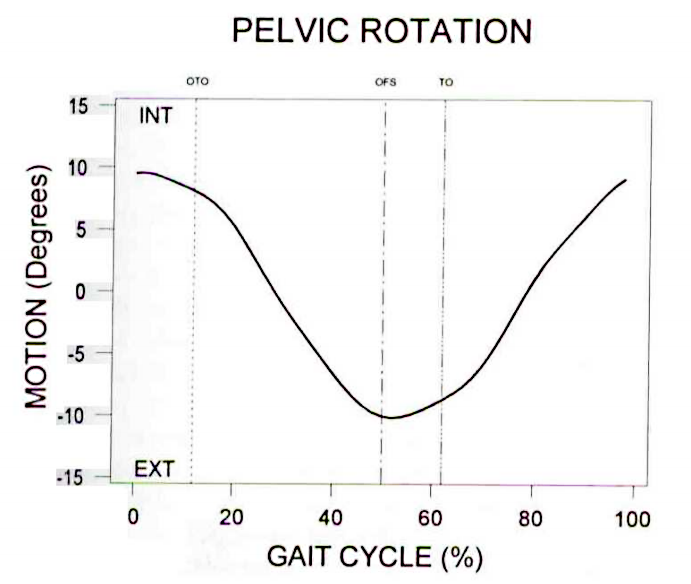
\includegraphics[width=7cm]{fig/pelvic_rotation.png}}}
\qquad
\subfloat{{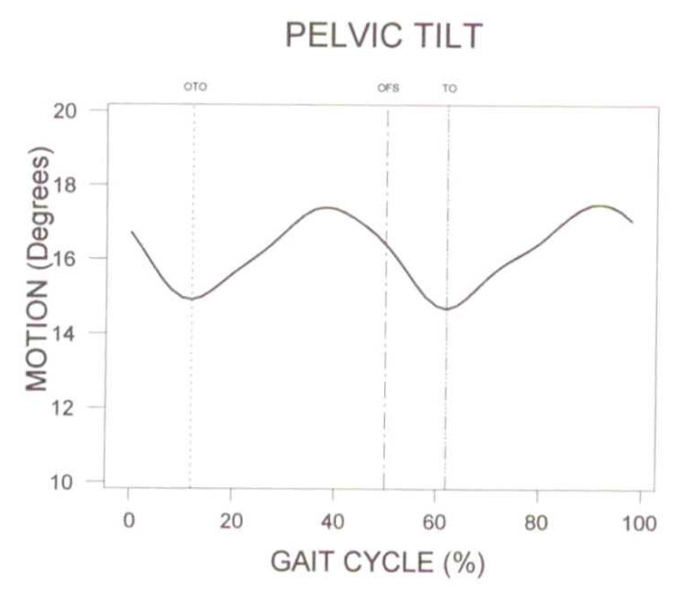
\includegraphics[width=7cm]{fig/pelvic_tilt.png}}}
\caption{Rotace a náklon pánve v průběhu krokového cyklu. Převzato z \cite{biomechanika_chuze}.} \label{pelvic kinematics}
\end{center}
\end{figure}

Pánev se vpřed nepohybuje po přímce, ale v ho\-ri\-zontální a sagitální rovině její trajektorie připomíná sinusoidu \cite{lin2014quantitative}. V sagitální rovině je maximální vertikální posun uprostřed stojné fáze a minimální ve fázi dvojí opory. Pro umožnění chůze po nerovném terénu budeme přizpůsobovat právě vertikální posun pánve. Použití Bézierových křivek nám umožní proložit krajní kontrolní body segmentů ma\-xi\-mem a minimem této trajektorie.

Při chůzi po nerovném terénu vertikální maximum pánve upravíme podle pozice stojné nohy, aby propnu\-tí kolena bylo nezměněno. Rozdíl ve výšce terénu v pozici předchozího a~následujícího umístění chodidla určuje změnu ve vertikálním maximu. Jestliže výška terénu je pro další krok nižší, snížíme o tuto hodnotu i vertikální minimum. Díky tomu může noha dosáhnout na cílovou pozici. Pokud je následující pozice nohy výše než předchozí, vertikální minimum neměníme, protože při chůzi do kopce se noha pokrčí v koleni a nemá problém dosáhnout na cílovou pozici. Výškový rozdíl pánve poté vyrovnáme až při narovnávání stojné nohy, viz obrázek \ref{fig:pelvis_vertical_uneven}.

\begin{figure}[h]
	\centering
	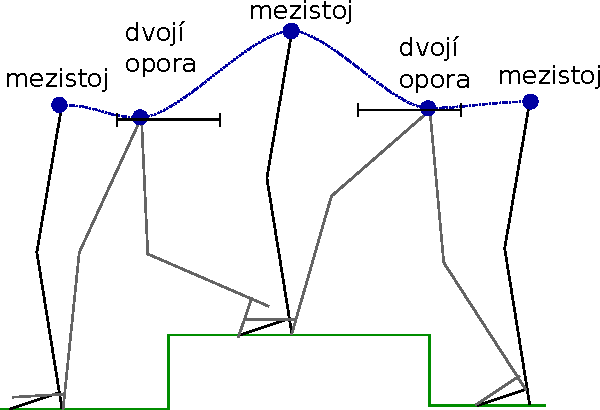
\includegraphics[width=0.5\linewidth]{fig/pelvis_vertical_uneven.pdf}
	\caption{Změna vertikální pozice pánve při chůzi po nerovném terénu. Obrázek také znázorňuje možné pozice pánve v dvojí opoře.}
	\label{fig:pelvis_vertical_uneven}
\end{figure}

Podobně jako při švihové fázi nohy se pánev pohybuje vpřed s variací v rychlosti. Pohyb se zrychluje se snižováním vertikální pozice a je nejrychlejší uprostřed dvojí opory, kdy je ki\-ne\-ti\-cká ener\-gie nejvyšší. Nejpomaleji se pánev pohybuje ve vertikálním maximu uprostřed stojné fáze. Posun pánve vpřed určujeme podle Beziérovy křivky, kterou jsme vytvořili podle grafů uvedených v \cite{chung}. Grafy se liší pro chůzi po rovině, z kopce, nebo do kopce. Vytvořili jsme jednu křivku pro chůzi po rovině a pro chůzi po nerovném terénu ji budeme upravovat podle pozice pánve ve dvojí opoře, viz obrázek \ref{fig:pelvis_speed}. Vertikální mi\-ni\-mum je v~čase vždy uprostřed dvojí opory. Pozice pánve ve dvojí opoře se ale může lišit. Pozicí pánve se dá manipulovat změnou křivky posunu, je nutné, aby pozice pánve v mezistoji byla vždy shodná. Z toho důvodu se křivka skládá ze dvou samostatných křivek. První určuje posun od dvojí opory k mezistoji a je upravena podle vzdálenosti mezi pozicemi pánve v těchto dvou okamžicích. Druhá určuje posun od mezistoje k dvojí opoře a je upravena obdobně. 

\begin{figure}[h]
	\centering
	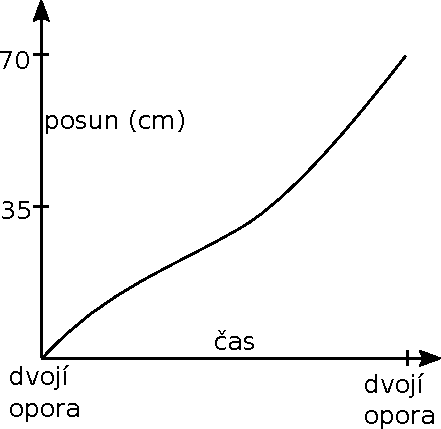
\includegraphics[width=0.3\linewidth]{fig/pelvis_speed_even.pdf}
	\qquad
	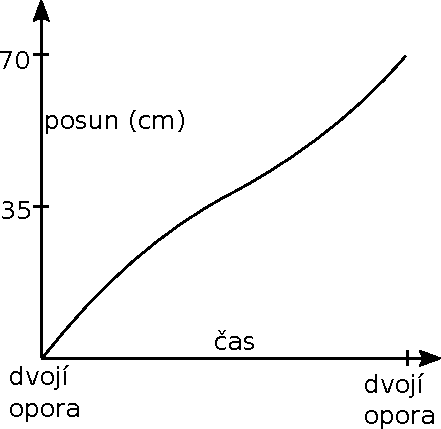
\includegraphics[width=0.3\linewidth]{fig/pelvis_speed_uneven.pdf}
	\caption{Posun pánve v čase mezi dvojími oporami. Vlevo je chůze po rovině, vpravo je křivka upravena podle pozice pánve při chůzi z kopce.}
	\label{fig:pelvis_speed}
\end{figure}

Pro určení pozice pánve ve vertikálním minimu je použit optimální přistup využívající rovnici z článku \cite{chung}. Vybírá se taková pozice pánve, aby úhlová akce\-le\-ra\-ce kloubů stojné nohy byla minimální. Protože chceme mít určenou trajektorii pánve již před určová\-ním trajektorie švihové nohy, určíme ji v okamžiku dvojí opory, než se švihová noha odrazí od~země.

Prvně se v rozsahu možných pozic určí úhlová akcelerace na pěti místech a poté se okolí místa s nejnižší akcelerací rozdělí na 5 dalších pozic, ze kterých se zase určí ta s~minimální akcelerací a ta je již finální. Výpočet úhlové akcelerace pro jednu pozici pánve vyžaduje následující úkony. Upravení jedné křivky posunu na vzdálenost mezi následujícím mezistojem a další dvojí oporou. A upravení druhé křivky posunu pro vzdálenost mezi další dvojí oporou a jí následujícím mezistojem. Dále je nutné určení trajektorie pánve v sagitální rovině v~závislosti na nerovnosti terénu. Poté se simuluje celý krok -- celkem 50krát. Z toho polovina simulačních kroků se provede pro část mezi mezistojem (MS) a dvojí oporou (DO). Pro aktuální stojnou nohu se pomocí inverzní kinematiky, a podle aktuální simulované fáze kroku, vypočítá pohyb kloubů nohy -- obdobně jako při samotné animaci chůze. V dvojí opoře se stojná noha změní na druhou a pro tuto druhou nohu se provede dalších 25 simulačních kroků. Při simulaci pohybu kloubů nohou je určován koeficient $c$ podle následující rovnice:

\begin{eqnarray}
c = \sum_{i=1}^{3} \mathbf{W}_i \int_{t_{MS}}^{t_{DO}}f_i(t)d^2t + \sum_{j=1}^{3} \mathbf{W}_j \int_{t_{DO}}^{t_{MS}}f_j(t)d^2t 
\label{eq:coefficient}
\end{eqnarray}
kde $f_i(t)$ je rotace $i$-tého kloubu v kinematickém řetězci pro danou pozici pánve a chodidla a čas $t$, $\mathbf{W}_i$ je váha $i$-tého kloubu.

Nakonec se z těch pozic, pro které stojná noha v průběhu celého kroku dosáhne na svoji pozici na zemi, vybere ta s nejmenším $c$ a je použita pro následující krok. V článku \cite{chung} určují také vertikální pozici pánve. Tu my máme určenou parametrem velikosti amplitudy v~sagitální rovině. Díky tomu máme menší množství pozic, které musíme prozkoumat a~máme lepší kontrolu nad vertikálním posunem. Ale pohyb není z hlediska akcelerace kloubů tolik optimální.

Důvod proč se ve dvojí opoře neprovádí simulace mezi aktuální pozicí a další dvojí oporou, ale provádí se od následujícího mezistoje k dalšímu mezistoji, je kvůli tomu jaká noha je stojná. V prvním případě by celou simulaci byla jedna stojná noha a zvolená pozice pánve by byla nevhodná, protože by nebrala v úvahu druhou nohu. Zatímco v druhém případě se stojná noha vystřídá a výsledná pozice tedy vyjadřuje kompromis mezi oběma nohami a pozice pánve je poté mnohem vhodnější. Simulace se neprovádí až ve chvíli, kdy je pánev v mezistoji, protože musíme mít určenou pozici pánve v další dvojí opoře již od~začátku švihové fáze, která začíná při odrazu nohy na konci dvojí opory. Zatímco mezistoj je až v polovině švihové fáze.

\subsection{Pohyb horní poloviny těla}
Lidský trup při chůzi vyrovnává rotaci pánve a natáčí ramena do opačného směru než pánev. Hlava směřuje vpřed a výrazně se nehýbe. V horizontální rovině je rotace ramen podobná rotaci pánve. Má opačnou amplitudu a dosahuje maxima před fází dvojí opory a během ní zůstává nezměněna \cite{ceccato2009comparison}. Tato rotace nevychází pouze z ramen, ale z celého trupu. V našem případě rotaci rovnoměrně rozkládáme mezi páteř, hruď a ramena. Hlava je rotována v~opačném směru a tato rotace je rozdělena mezi hlavu a krk tak, že hlava směřuje vpřed.  

Ve frontální rovině rotaci pánve vyrovnáváme tak, aby pozice krku byla ve svislé poloze s pánví (obrázek \ref{fig:vyrovnani_patere}). Dále je natočena hlava podle úhlu $\delta$, aby byla rovnoběžná se svislou osou. Úhel potřebné rotace páteře a hrudi $\alpha$ pro danou rotaci pánve $\theta$ je získán vyřešením následující rovnice:
\begin{eqnarray}
l_1 \sin(\theta) = l_2 \sin(\theta + \alpha) + l_3 \sin(\theta + 2\alpha)
\label{eq:spine_equation}
\end{eqnarray}
Tato rovnice je řešena numericky pomocí metody Regula Falsi.

\begin{figure}[h]
	\centering
	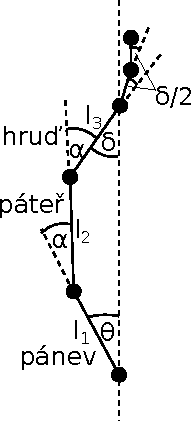
\includegraphics[width=0.17\linewidth]{fig/vyrovnani_patere.pdf}
	\caption{Pohyb trupu a hlavy v závislosti na rotaci pánve ve frontální rovině. Trup je rotován tak, aby pozice krku byla v ose nad pánví.}
	\label{fig:vyrovnani_patere}
\end{figure}

\subsubsection{Pohyb rukou}
O pohyb rukou se stará třída \texttt{Arm}. Obdobně jako třída \texttt{Leg} obsahuje metodu \texttt{update}, které je předáván čas od posledního snímku animace. Pohyb rukou je ale výrazně jednodušší. Inverzní kinematika je využita pouze jednou při inicializaci pro nastavení rukou do výchozí pozice podél těla. Inverzní kinematika je řešená stejně jako pro nohy, ale místo stehenní kosti se používá paže a místo holenní kosti předloktí. 

Dále je každý snímek rotována paže a předloktí pomocí Bézierových křivek. Prvně je paže rotována okolo svislé osy o aktuální rotaci pánve, díky tomu bude ruka směřovat vpřed. Poté je vyrovnán úklon pánve, aby ruka směřovala dolů. Nakonec je rotována paže a~loket podle křivek na obrázku \ref{fig:shoulder_elbow}. Ruce se pohybují v opačném směru než nohy, tzn. jsou v~největším rozpětí ve fázi dvojí opory.

\begin{figure}[h]
	\centering
	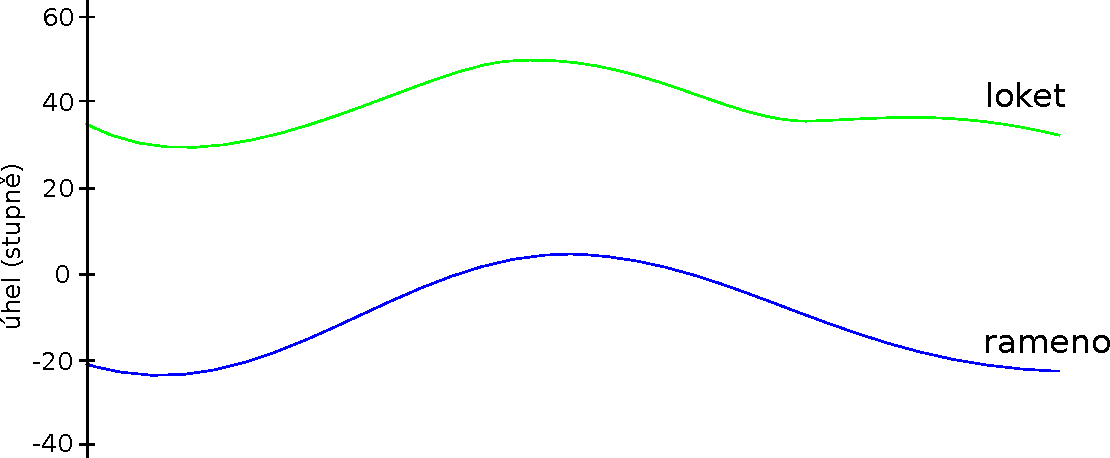
\includegraphics[width=0.7\linewidth]{fig/shoulder_elbow.pdf}
	\caption{Křivky pro rotaci v rameni a v lokti, grafy jsou aproximovány podle \cite{ceccato2009comparison}.}
	\label{fig:shoulder_elbow}
\end{figure}

\section{Nastavování parametrů}
Systém umožňuje nastavování parametrů chůze v reál\-ném čase. Pro parametry jako je pozice a rotace pánve a rukou je možné zvětšovat amplitudu Bézierových křivek. Aby byl pohyb při změně parametrů plynulý, musíme zajistit návaznost segmentů. Toho dosáhneme tak, že změníme hodnotu třetího a čtvrtého kontrolního bodu následujícího segmentu od aktuální pozice, viz obrázek \ref{fig:zmena_parametru_tilt}. A dále změníme hodnoty všech následující kontrolních bodů.

\begin{figure}[h]
	\centering
	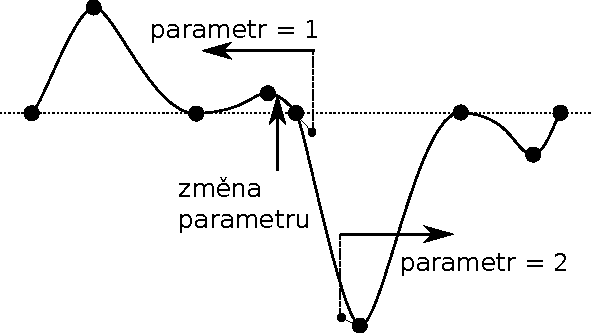
\includegraphics[width=0.5\linewidth]{fig/zmena_parametru_tilt.pdf}
	\caption{Bézierova křivka určující úklon (rotaci ve frontální rovině) pánve. Při změně parametru jsou změněny kontrolní body začínající třetím kontrolním bodem následujícího segmentu.}
	\label{fig:zmena_parametru_tilt}
\end{figure}

Na nejvyšší úrovni kontroly umožňujeme specifikovat rychlost chůze. Výzkum \cite{orendurff2004effect} ukazuje, že se zvyšující se rychlostí chůze se snižuje pohyb pánve v horizontální rovině a zvyšuje ve vertikální rovině. Také se zvyšuje délka kroku, počet kroků za minutu a šířka kroku. Aby nohy dosáhly na požadovanou délku kroku, snižujeme i maximální výšku pánve, přestože se v článku nezmiňuje.

Dále se dají parametry nastavovat samostatně. Pro pohyb pánve je možné měnit amplitudy křivek pro rotaci, úklon, náklon pánve, ale také horizontální a vertikální posun. Kromě toho je možné určit maximální výšku pánve, předklon trupu a pozici pánve v mezistoji, tedy posun pánve vůči chodidlu stojné nohy v maximu vertikálního pohybu pánve. 

Pro pohyb nohou je možné nastavit délku a šířku kroku. Dále úhel vytočení chodidla, který se mění rotací referenčního vektoru při řešení inverzní kinematiky. Výška zvedání kolen se dá měnit zvyšováním středu trajektorie švihové nohy. Obdobně jako při úpravě trajektorie kdy se noha nachází pod terénem. Je také možné změnit dobu trvání kroku.

Pro pohyb rukou je možné měnit amplitudy křivek pro rotaci v rameni a v lokti. Dále je možné měnit rozpřáhnutí rukou a maximální napnutí loktu. A konečně je možné měnit váhy pro kyčel, koleno a kotník při určování vhodné pozice pánve v dvojí opoře.

Pro nastavování parametrů slouží grafické uživatelské rozhraní. Pro jeho tvorbu je využita knihovna ImGui. Pro změnu parametrů slouží posuvníky. Pomocí tlačítek je možné vybrat některou z přednastavených chůzí. Dále je možné přecházet mezi různými modely a terény. Pomocí grafického uživatelského rozhraní jsou také zobrazeny zajímavé křivky, které se přizpůsobují nerovnému terénu. Na obrázku \ref{fig:screen} je možné vidět výslednou aplikaci i~s~grafickým uživatelským rozhraním. Pro ukázku výsledné aplikace bylo také vytvořeno video\protect\footnotemark.

\footnotetext{Dostupné z \url{https://youtu.be/Z5Qckdr9yDI}}

\begin{figure}[h]
	\centering
	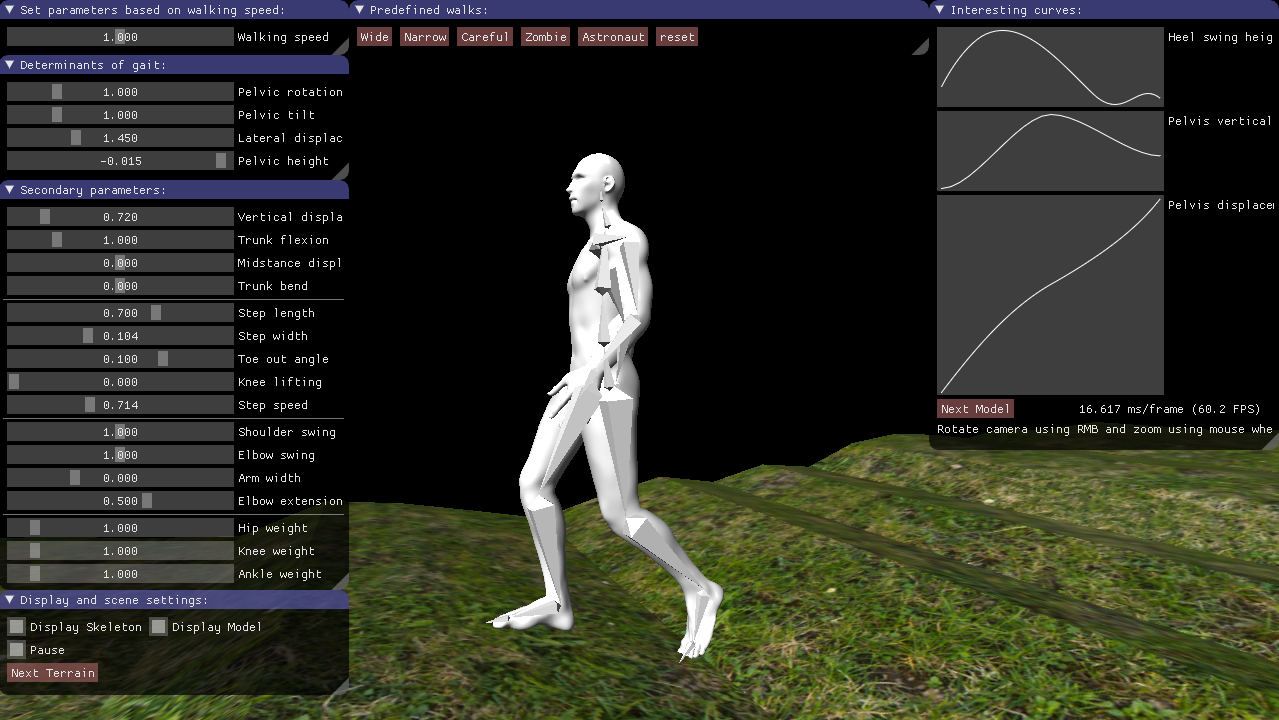
\includegraphics[width=1.0\linewidth]{fig/screen.png}
	\caption{Výsledná aplikace s grafickým uživatelským rozhraním při chůzi po nerovném terénu.}
	\label{fig:screen}
\end{figure}

\section{Měření rychlosti}
Aplikaci jsme testovali na notebooku Asus K53SV s Intel Core i5 procesorem a GeForce GT 540M grafic\-kou kartou. Vykreslení jednoho snímku trvá průměrně 5ms. Tato doba je nezávislá na komplexnosti terénu. V průběhu jednoho kroku mají dva snímky výrazně delší dobu výpočtu -- když se určuje trajektorie pánve a upravuje trajektorie nohy ve švihové fázi. Při nedostatku výpočetního výkonu může v těchto snímcích docházet k neplynulosti animace. V tabulce \ref{tab:measure_table} je uvedeno kolik procent z celkového času zabírají některé části aplikace.

Pro porovnání podobný systém \cite{chung}, který je také procedurální a řeší chůzi po nerovném terénu, je scho\-pen vypočítat 3.75 kroků za vteřinu s 10 snímky na krok na procesoru Pentium-II 300 MHz. Tento systém neřeší horní polovinu těla a zobrazování trojrozměrné\-ho mo\-delu.

\begin{table}[h]
	\vskip6pt
	\caption{Podíl částí řešení na celkovém času, který aplikace stráví na CPU. Části řešení se nevylučují.}
	\centering
	\begin{tabular}{llr}
		\toprule
		Funkce & Procento celkového času \\
		\midrule
		Vykreslování scény & $25$ \\
		Vykreslování GUI & $35$ \\
		Řešení inverzní kinematiky & $5$ \\
		Určení pozice pánve & $10$ \\
		Vyhodnocování křivek & $3$ \\
		Řešení rukou & $0.6$ \\
		Řešení nohou & $5$ \\
		Řešení páteře & $0.08$ \\
		\bottomrule
	\end{tabular}
	\label{tab:measure_table}
\end{table}

\chapter{Závěr}
V této práci jsme se zabývali implementací animace lidské chůze s nastavitelnými parametry a možností chůze po nerovném terénu. Byla představena skeletální animace, metody tvorby animace a nastíněny možné přístupy ke tvorbě animace lidské chůze. Definovali jsme inverzní kinematiku a popsali některé metody jejich řešení. Dále byly popsány fáze lidské chůze a~dvě existující řešení procedurální animace chůze. Následně bylo popsáno načtení a zobrazení modelu a samotná implementace animace. Nakonec byla změřena rychlost aplikace.

Podařilo se nám za využití interpolačních křivek a inverzní kinematiky vytvořit realistickou animaci lidské chůze. K tomu jsme se inspirovali existujícími řešeními pro pohyb pánve a využili vlastní řešení pro pohyb horní poloviny těla a nohou. Vytvořená animace umožňuje chůzi po nerovném terénu, kde ale může při velkém sklonu terénu docházet k nepřirozenému ohybu v kotníku. Výpočet animace je rychlý díky využití analytického řešení inverzní kinematiky. Pomocí parametrů chůze se dají nastavit velmi odlišné a specifické animace chůze.

O této práci jsem také napsal článek, který jsem prezentoval na studentské konferenci Excel@FIT 2016, a za který jsem byl oceněn odborným panelem. Výsledky práce by mohli být použity při tvorbě počítačových her. V takovém případě by bylo vhodné implementovat animace iniciace a zastavení chůze a případně i animace běhu. Také by po implementaci exportu animace do souborového formátu bylo možné práci využít pro tvorbu animace klíčových snímků.

%=========================================================================
 % viz. obsah.tex

  % Pouzita literatura
  % ----------------------------------------------
\ifslovak
  \makeatletter
  \def\@openbib@code{\addcontentsline{toc}{chapter}{Literatúra}}
  \makeatother
  \bibliographystyle{czechiso}
\else
  \ifczech
    \makeatletter
    \def\@openbib@code{\addcontentsline{toc}{chapter}{Literatura}}
    \makeatother
    \bibliographystyle{czechiso}
  \else 
    \makeatletter
    \def\@openbib@code{\addcontentsline{toc}{chapter}{Bibliography}}
    \makeatother
    \bibliographystyle{plain}
  %  \bibliographystyle{alpha}
  \fi
\fi
  \begin{flushleft}
  \bibliography{literatura} % viz. literatura.bib
  \end{flushleft}

  % Prilohy
  % ---------------------------------------------
  \appendix
\ifczech
  \renewcommand{\appendixpagename}{Přílohy}
  \renewcommand{\appendixtocname}{Přílohy}
  \renewcommand{\appendixname}{Příloha}
\fi
\ifslovak
  \renewcommand{\appendixpagename}{Prílohy}
  \renewcommand{\appendixtocname}{Prílohy}
  \renewcommand{\appendixname}{Príloha}
\fi
  \appendixpage

\ifslovak
  \section*{Zoznam príloh}
  \addcontentsline{toc}{section}{Zoznam príloh}
\else
  \ifczech
    \section*{Seznam příloh}
    \addcontentsline{toc}{section}{Seznam příloh}
  \else
    \section*{List of Appendices}
    \addcontentsline{toc}{section}{List of Appendices}
  \fi
\fi
  \startcontents[chapters]
  \printcontents[chapters]{l}{0}{\setcounter{tocdepth}{2}}
  \chapter{Obsah CD}
\begin{itemize}

\item \textbf{tex/ - } 
Obsahuje zdrojový tvar písemné zprávy v \LaTeX u. Překlad je možný pomocí \texttt{\$make}. Případně v Texmakeru pomocí pdflatex + bibtex + pdflatex + pdflatex. Adresář \texttt{fig/} obsahuje obrázky použité v písemné zprávě.

\item \textbf{proceduralni\_animace\_lidske\_chuze.pdf - }
Přeložená písemná zpráva ve formátu pdf.

\item \textbf{human\_walk/ - }
Obsahuje \textit{solution} pro Visual Studio 2013 se zdrojovými kódy aplikace. Ve Visual studiu se aplikace přeloží pomocí Build/Build Solution (ctrl + F7) a spustí pomocí Debug/Start Debugging (F5). Aplikace vyžaduje podporu OpenGL 3.1. Zdrojové kódy jsou v podadresáři \texttt{human\_walk/source/}. V rámci práce nebyly vytvořeny soubory \texttt{imconfig}, \texttt{imgui}, \texttt{imgui\_demo}, \texttt{imgui\_draw}, \texttt{imgui\_impl\_sdl\_gl3}, \texttt{imgui\_internal}, \texttt{stb\_rect\_pack}, \texttt{stb\_textedit}, \texttt{stb\_truetype} a \texttt{lodepng}.

\item \textbf{Release/ - }
Obsahuje přeloženou aplikaci pro Windows a další soubory potřebné pro její běh.

\item \textbf{video.mp4 - }
Video s prezentací projektu. Dostupné také z \url{https://youtu.be/Z5Qckdr9yDI}

\item \textbf{skeleton.dae - }
Kostra nad kterou aplikace pracuje.

\end{itemize}

\chapter{Manuál}
Po načtení aplikace se zobrazí první model na nerovném terénu. Pro změnu parametrů je možné použít grafické uživatelské rozhraní, jehož okna je možné skrýt dvojklikem na jejich lišty. Pomocí tlačítka \texttt{Next terrain} je možné přepínat mezi nerovným, schodovitým a rovným terénem. Tlačítko \texttt{Next model} přepne na další scénu s  jiným modelem.
Rotace kamery se ovládá pravým tlačítkem myši. Kolečkem myši je možné přibližovat a oddalovat kameru. Kamera se pohybuje spolu s modelem.
Některé funkce je také možné ovládat pomocí tlačítek na klávesnici: 
\begin{itemize} \itemsep1pt \parskip0pt \parsep0pt
\item[] \textbf{mezerník} - pozastavení/spuštění animace
\item[] \textbf{tabulátor} - přepínání mezi scénami s různými modely
\item[] \textbf{1} - vypnutí/zapnutí zobrazení kostry
\item[] \textbf{2} - vypnutí/zapnutí zobrazení modelu
\item[] \textbf{+} - přiblížení kamery
\item[] \textbf{-} - oddálení kamery
\end{itemize}

Pro připravení modelu pro běh v aplikaci je potřeba k němu připojit přiloženou kostru např. pomocí automatického přiřazení vah a vyexportovat v Blenderu do formátu COLLADA.

%\chapter{Manual}
%\chapter{Konfigrační soubor}
%\chapter{RelaxNG Schéma konfiguračního soboru}
%\chapter{Plakat}

 % viz. prilohy.tex
\end{document}
